\chapter{Dataset Examination} \label{sec:Dataset}

\section{Friends} \label{sec:Dataset_Friends}

The number of friends users in the dataset have can be seen in Figure \ref{fig:Dataset_HistFriends}. Outliers\footnote[2]{Values outside of the interquartile range multiplied by some scaling value were considered to be outliers \cite{Seo2006_Outliers}. The scaling value was chosen so as to balance visual and statistical clarity.} have been excluded from the aforementioned histogram for the sake of visual clarity and, as such, users with more than 119 friends, 2\% of all users, are not shown. The mean number of friends users have is 28.7 (\textit{SD} = 46.9) and the median is 16. As mentioned in section \ref{sec:BG_Dataset}, users without any friends have been excluded.

Users in the dataset tend to have a modest number of friends with 75\% of users having 7 or more friends, although users with a single friend are the most common occurrence.

\begin{figure}[ht]
    \centering
    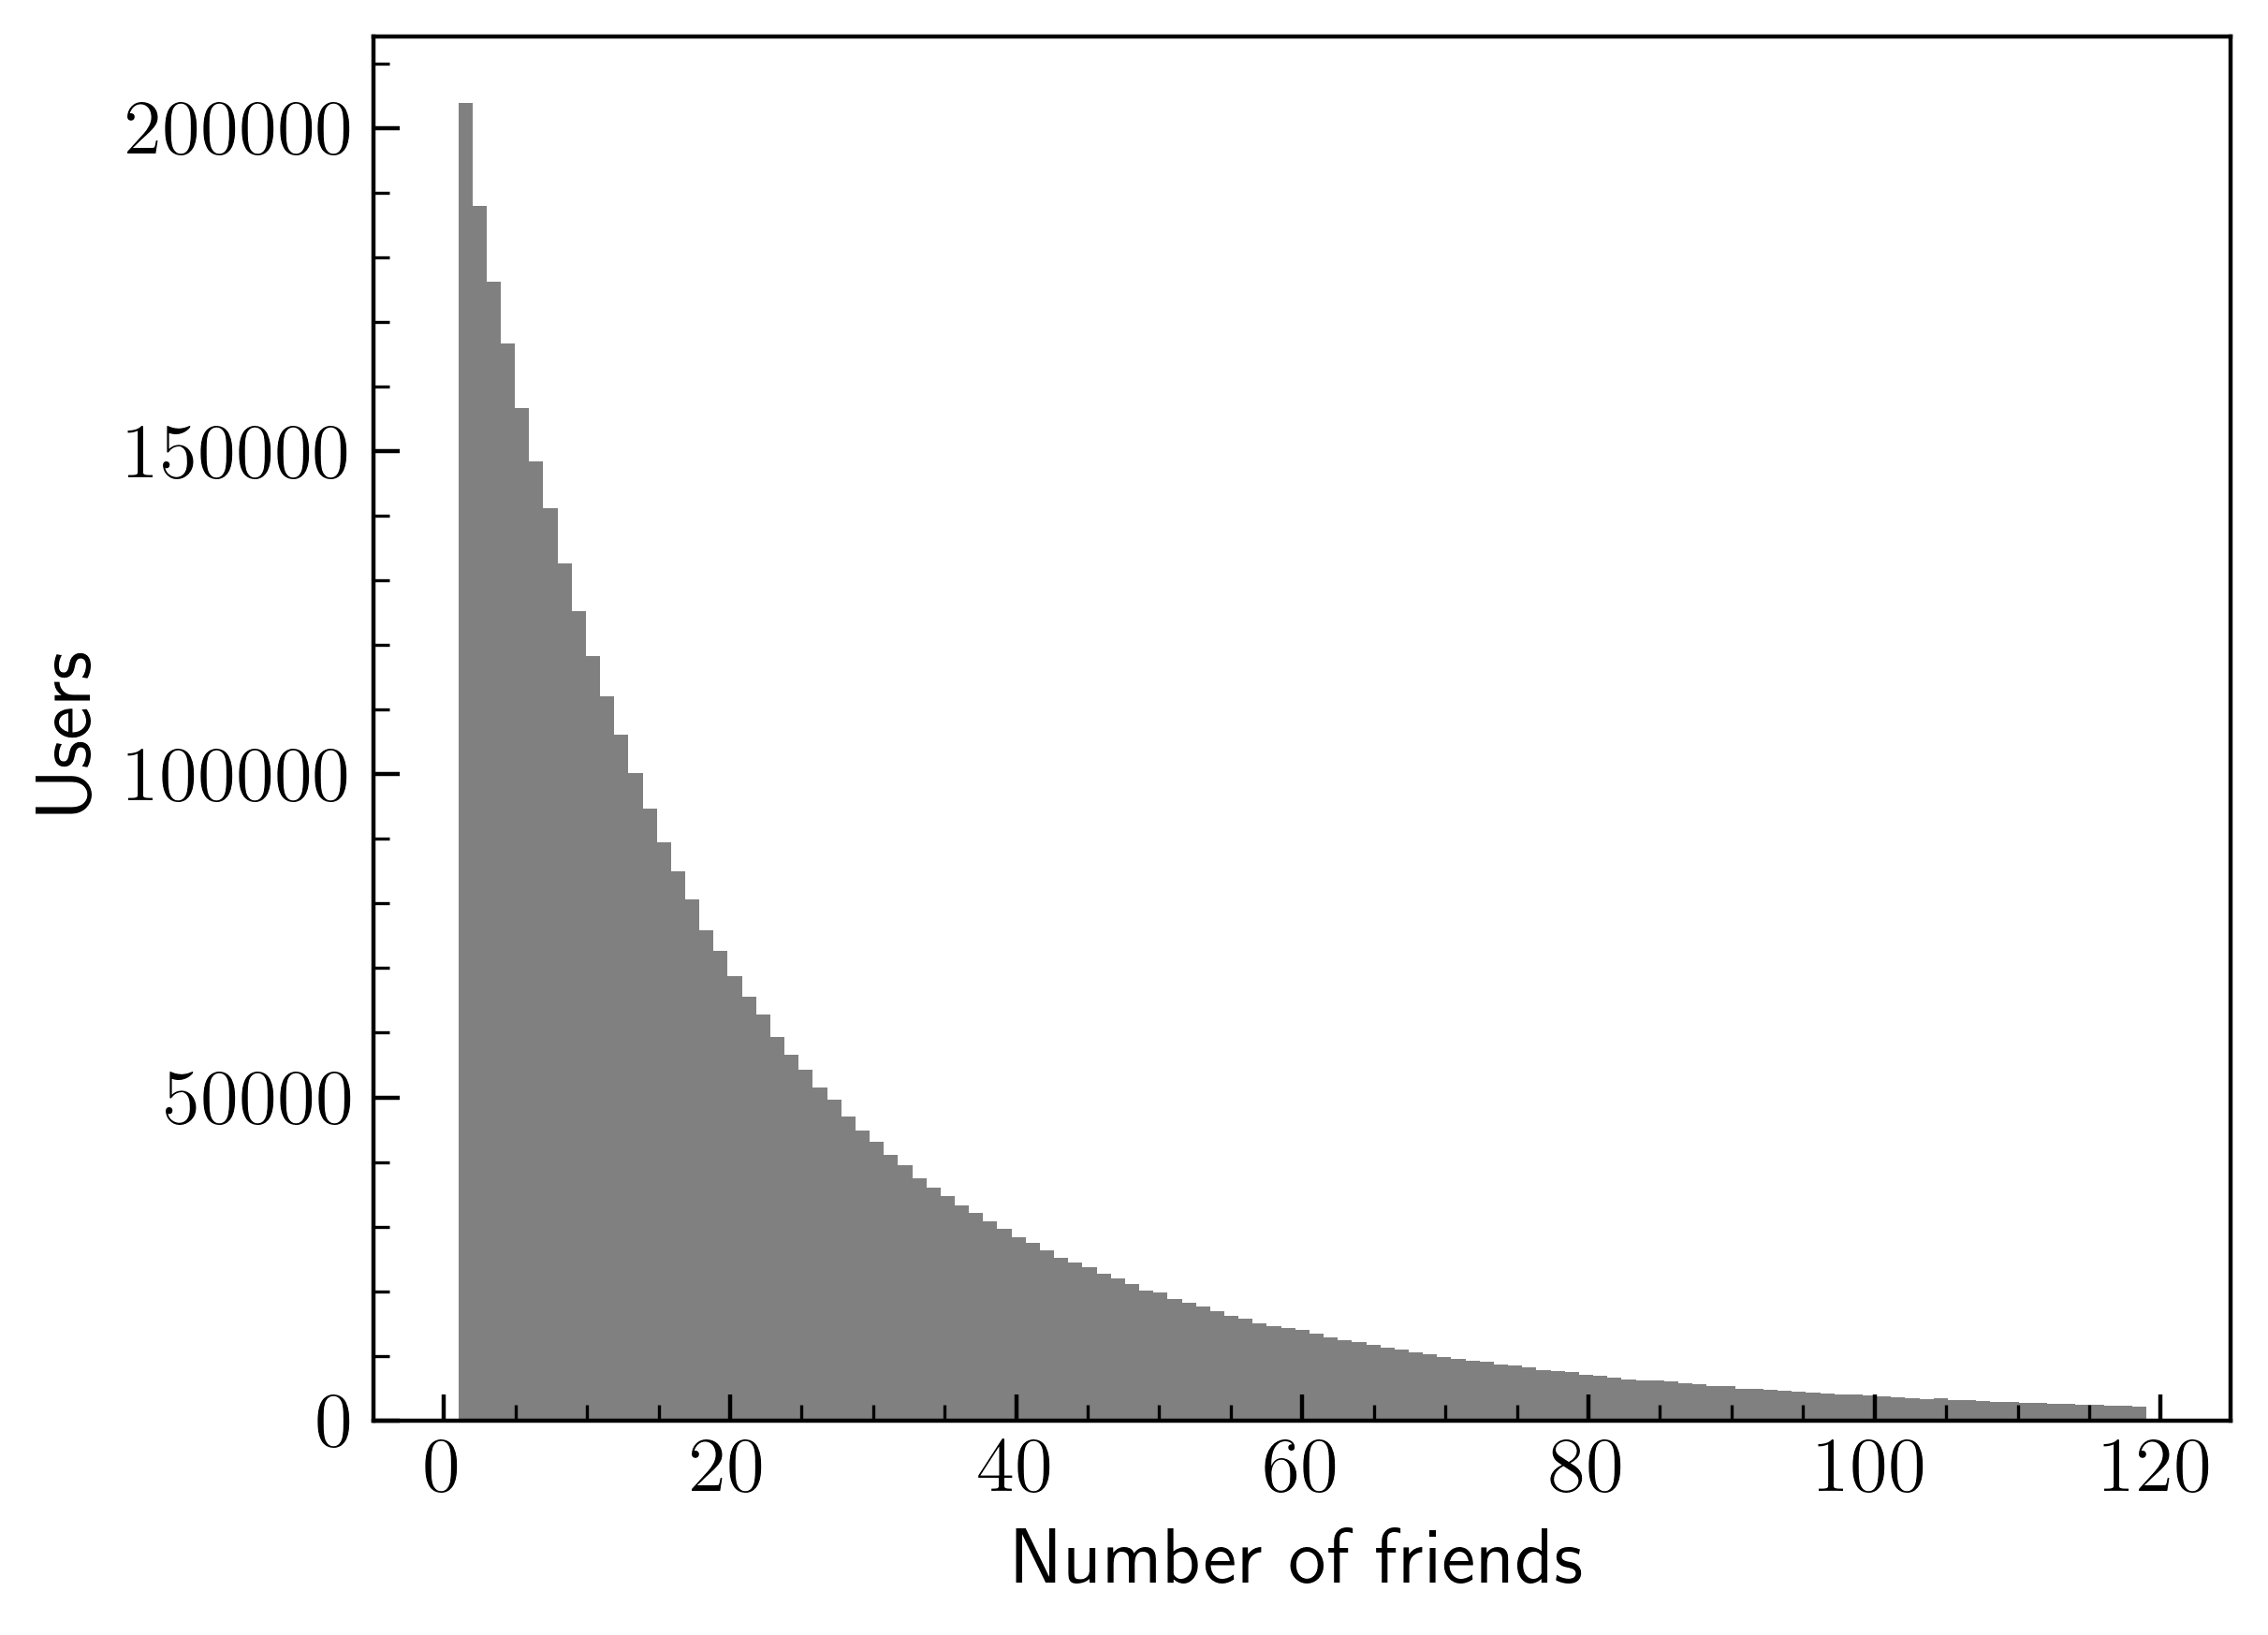
\includegraphics[scale=0.55]{figures/03_dataset/01_hist_friends.png}
    \caption{Number of friends that users have.}
    \label{fig:Dataset_HistFriends}
\end{figure}

\section{Groups} \label{sec:Dataset_Groups}

The number of members groups in the dataset have as well as the number of groups users are members of can be seen in Figure \ref{fig:Dataset_HistsGroups}. Groups with more than 12 members, 5\% of all groups, and users who are members of more than 45 groups, 5\% of all users, have been excluded from their respective histograms. The mean number of members groups have is 8.9 (\textit{SD} = 339.2) and the median is 1. The mean number of groups users are members of is 12.8 (\textit{SD} = 37.2) and the median is 4. Due to the nature in which the data was gathered, the values given for the number of members that groups have is limited to those users included in the dataset as opposed to all users on Steam.

The majority of groups in the dataset only contain a single member and most users tend not to be members of many, if any, groups.

\begin{figure}[ht]
    \centering
    \begin{subfigure}[ht]{0.49\textwidth}
        \centering
        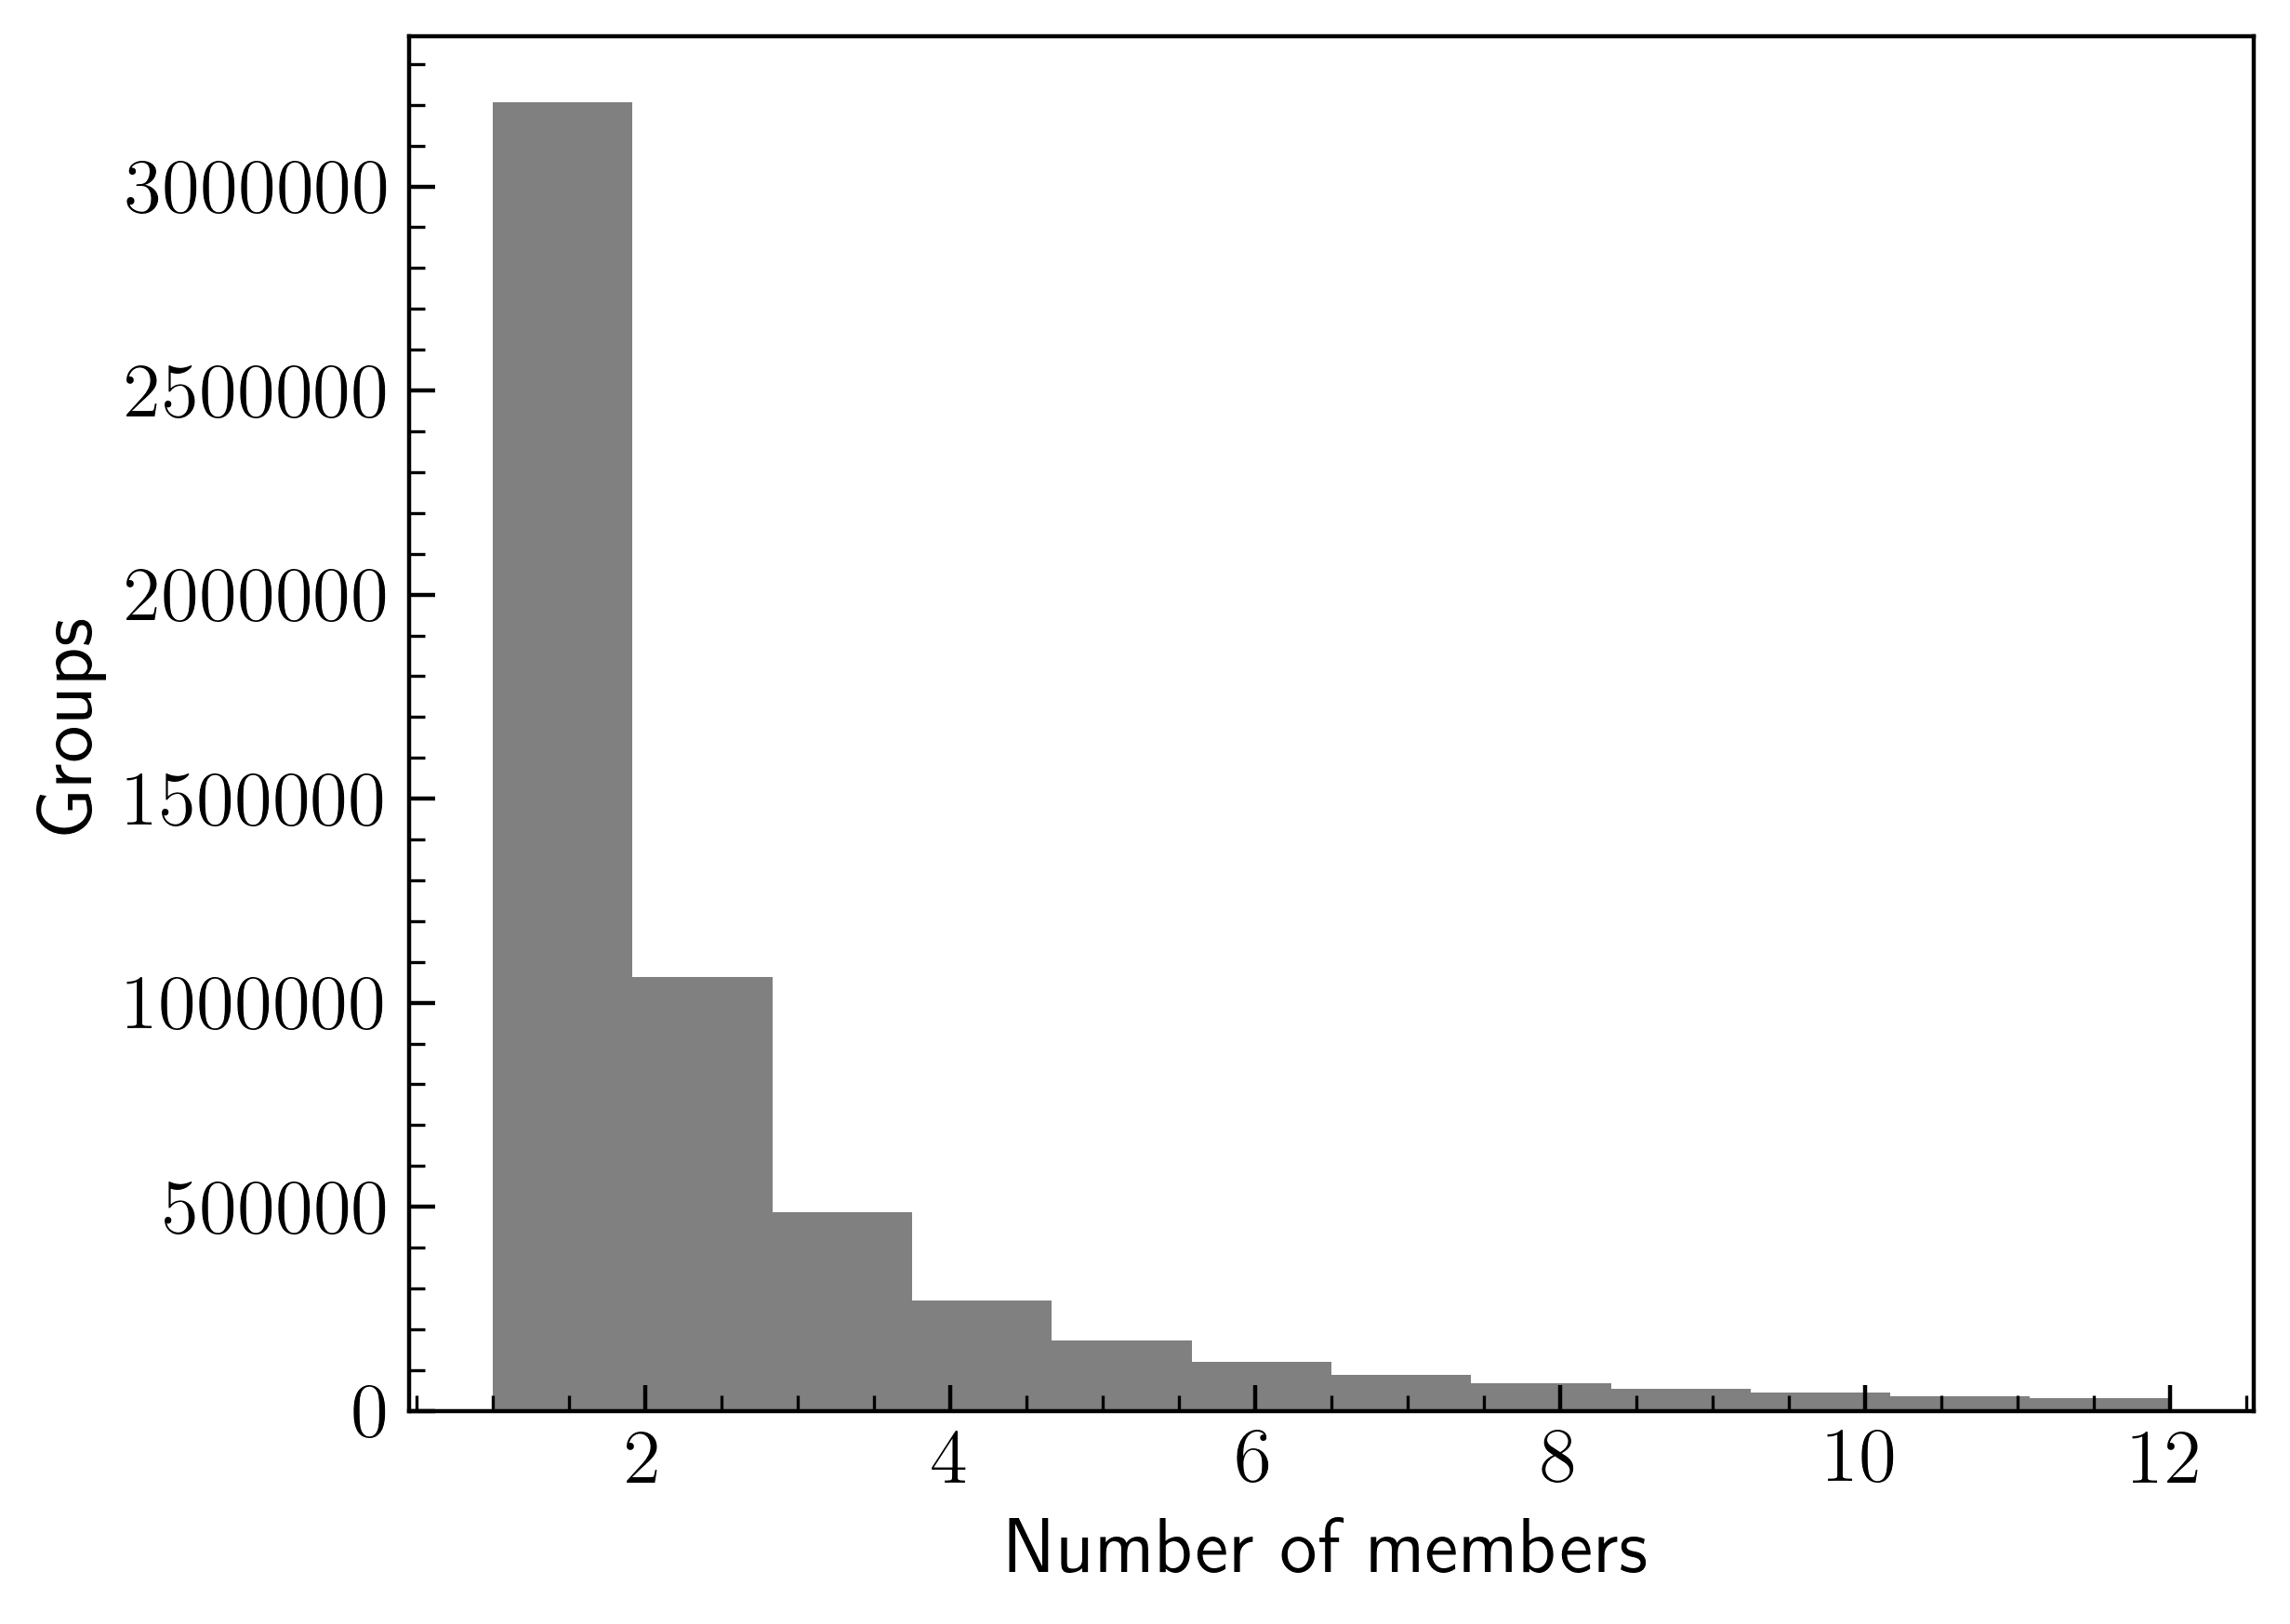
\includegraphics[width=\textwidth]{figures/03_dataset/02_hist_group_users.png}
        \caption{Number of members that groups have.}
        \label{fig:Dataset_HistGroupUsers}
    \end{subfigure}
    \hfill
    \begin{subfigure}[ht]{0.49\textwidth}
        \centering
        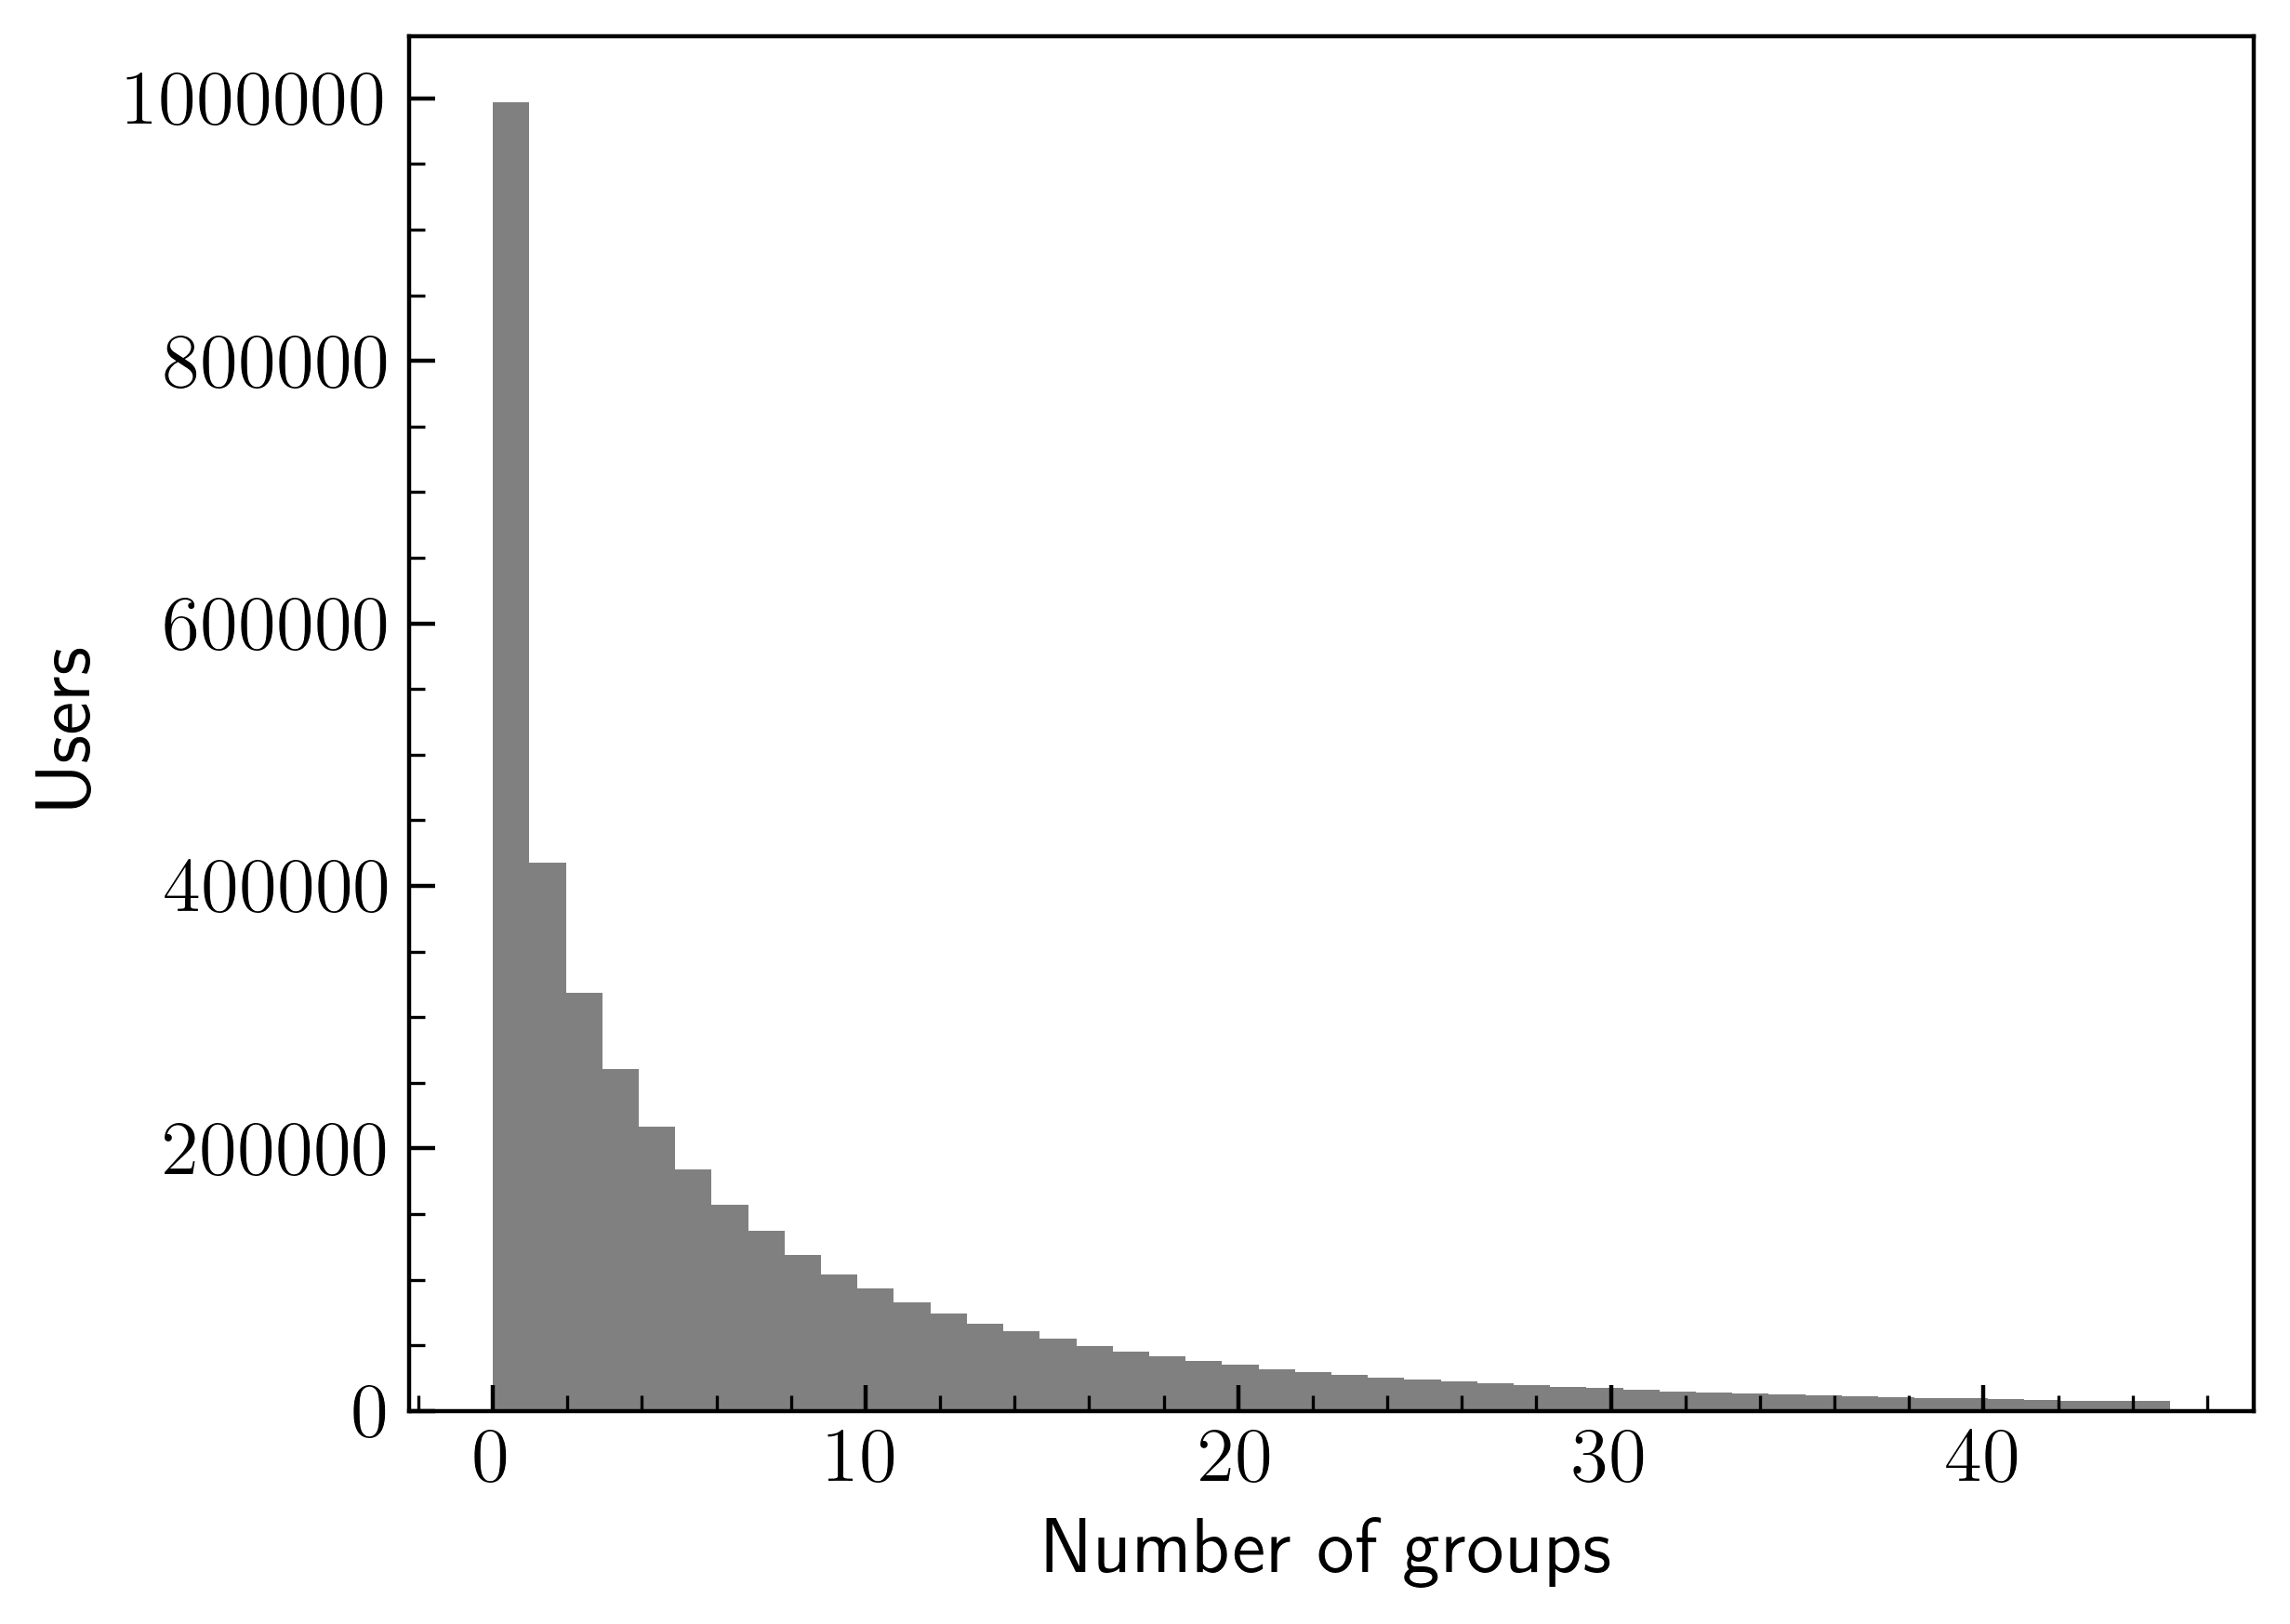
\includegraphics[width=\textwidth]{figures/03_dataset/03_hist_user_groups.png}
        \caption{Number of groups that users are members of.}
        \label{fig:Dataset_HistUserGroups}
    \end{subfigure}
    \caption{Group membership distributions.}
    \label{fig:Dataset_HistsGroups}
\end{figure}

\section{Reviews} \label{sec:Dataset_Reviews}

\subsection{Number of Reviews}

The number of reviews users have written as well as the number of reviews that games have can be seen in Figure \ref{fig:Dataset_HistsReviews}. Users who have written more than 22 reviews, 3\% of all users, and games with more than 161 reviews, 8\% of all games, have been excluded from their respective histograms. The mean number of reviews users have written is 4.6 (\textit{SD} = 16.8) and the median is 2. The mean number of reviews games have is 165.5 (\textit{SD} = 3611.1) and the median is 7. As was the case with groups, the values given for the number of reviews that games have is limited to those reviews included in the dataset as opposed to all reviews on Steam.

Most users in the dataset have only written a single review and 75\% of users have written 4 reviews or fewer. Similarly, most games in the dataset have only had a single review written for them.

\begin{figure}[ht]
    \centering
    \begin{subfigure}[ht]{0.49\textwidth}
        \centering
        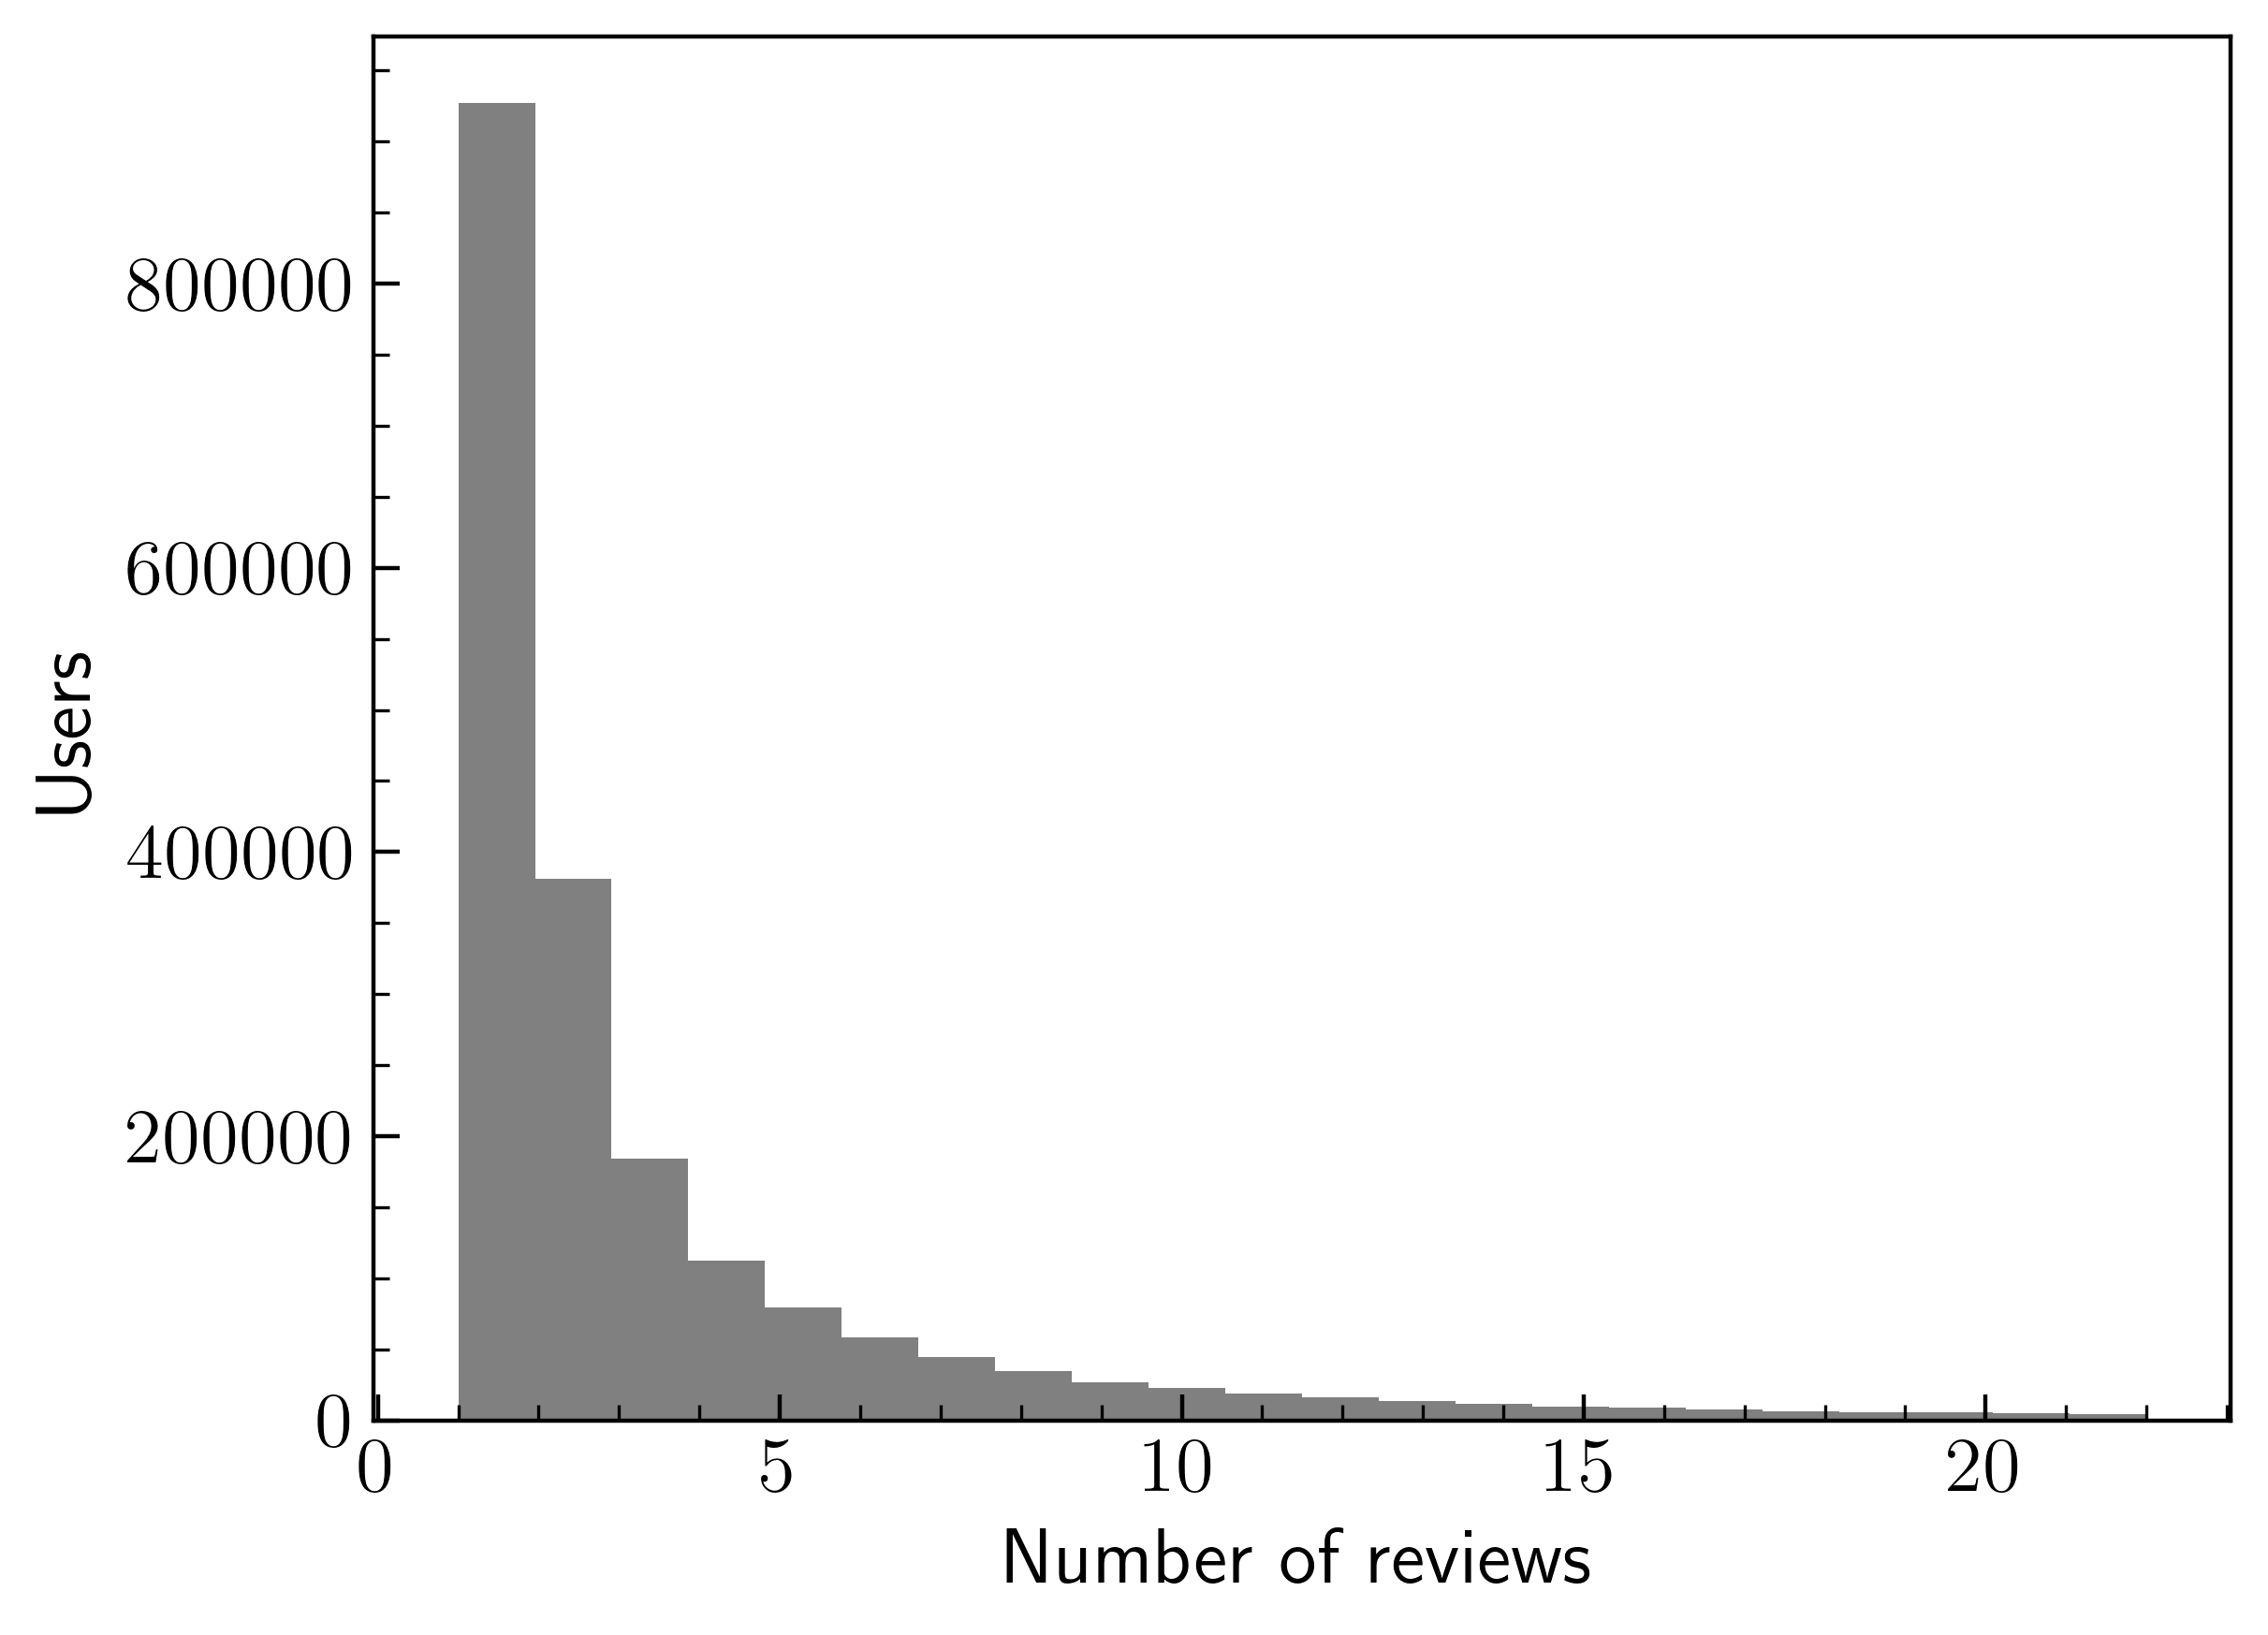
\includegraphics[width=\textwidth]{figures/03_dataset/04_hist_user_reviews.png}
        \caption{Number of reviews users wrote.}
        \label{fig:Dataset_HistUserReviews}
    \end{subfigure}
    \hfill
    \begin{subfigure}[ht]{0.49\textwidth}
        \centering
        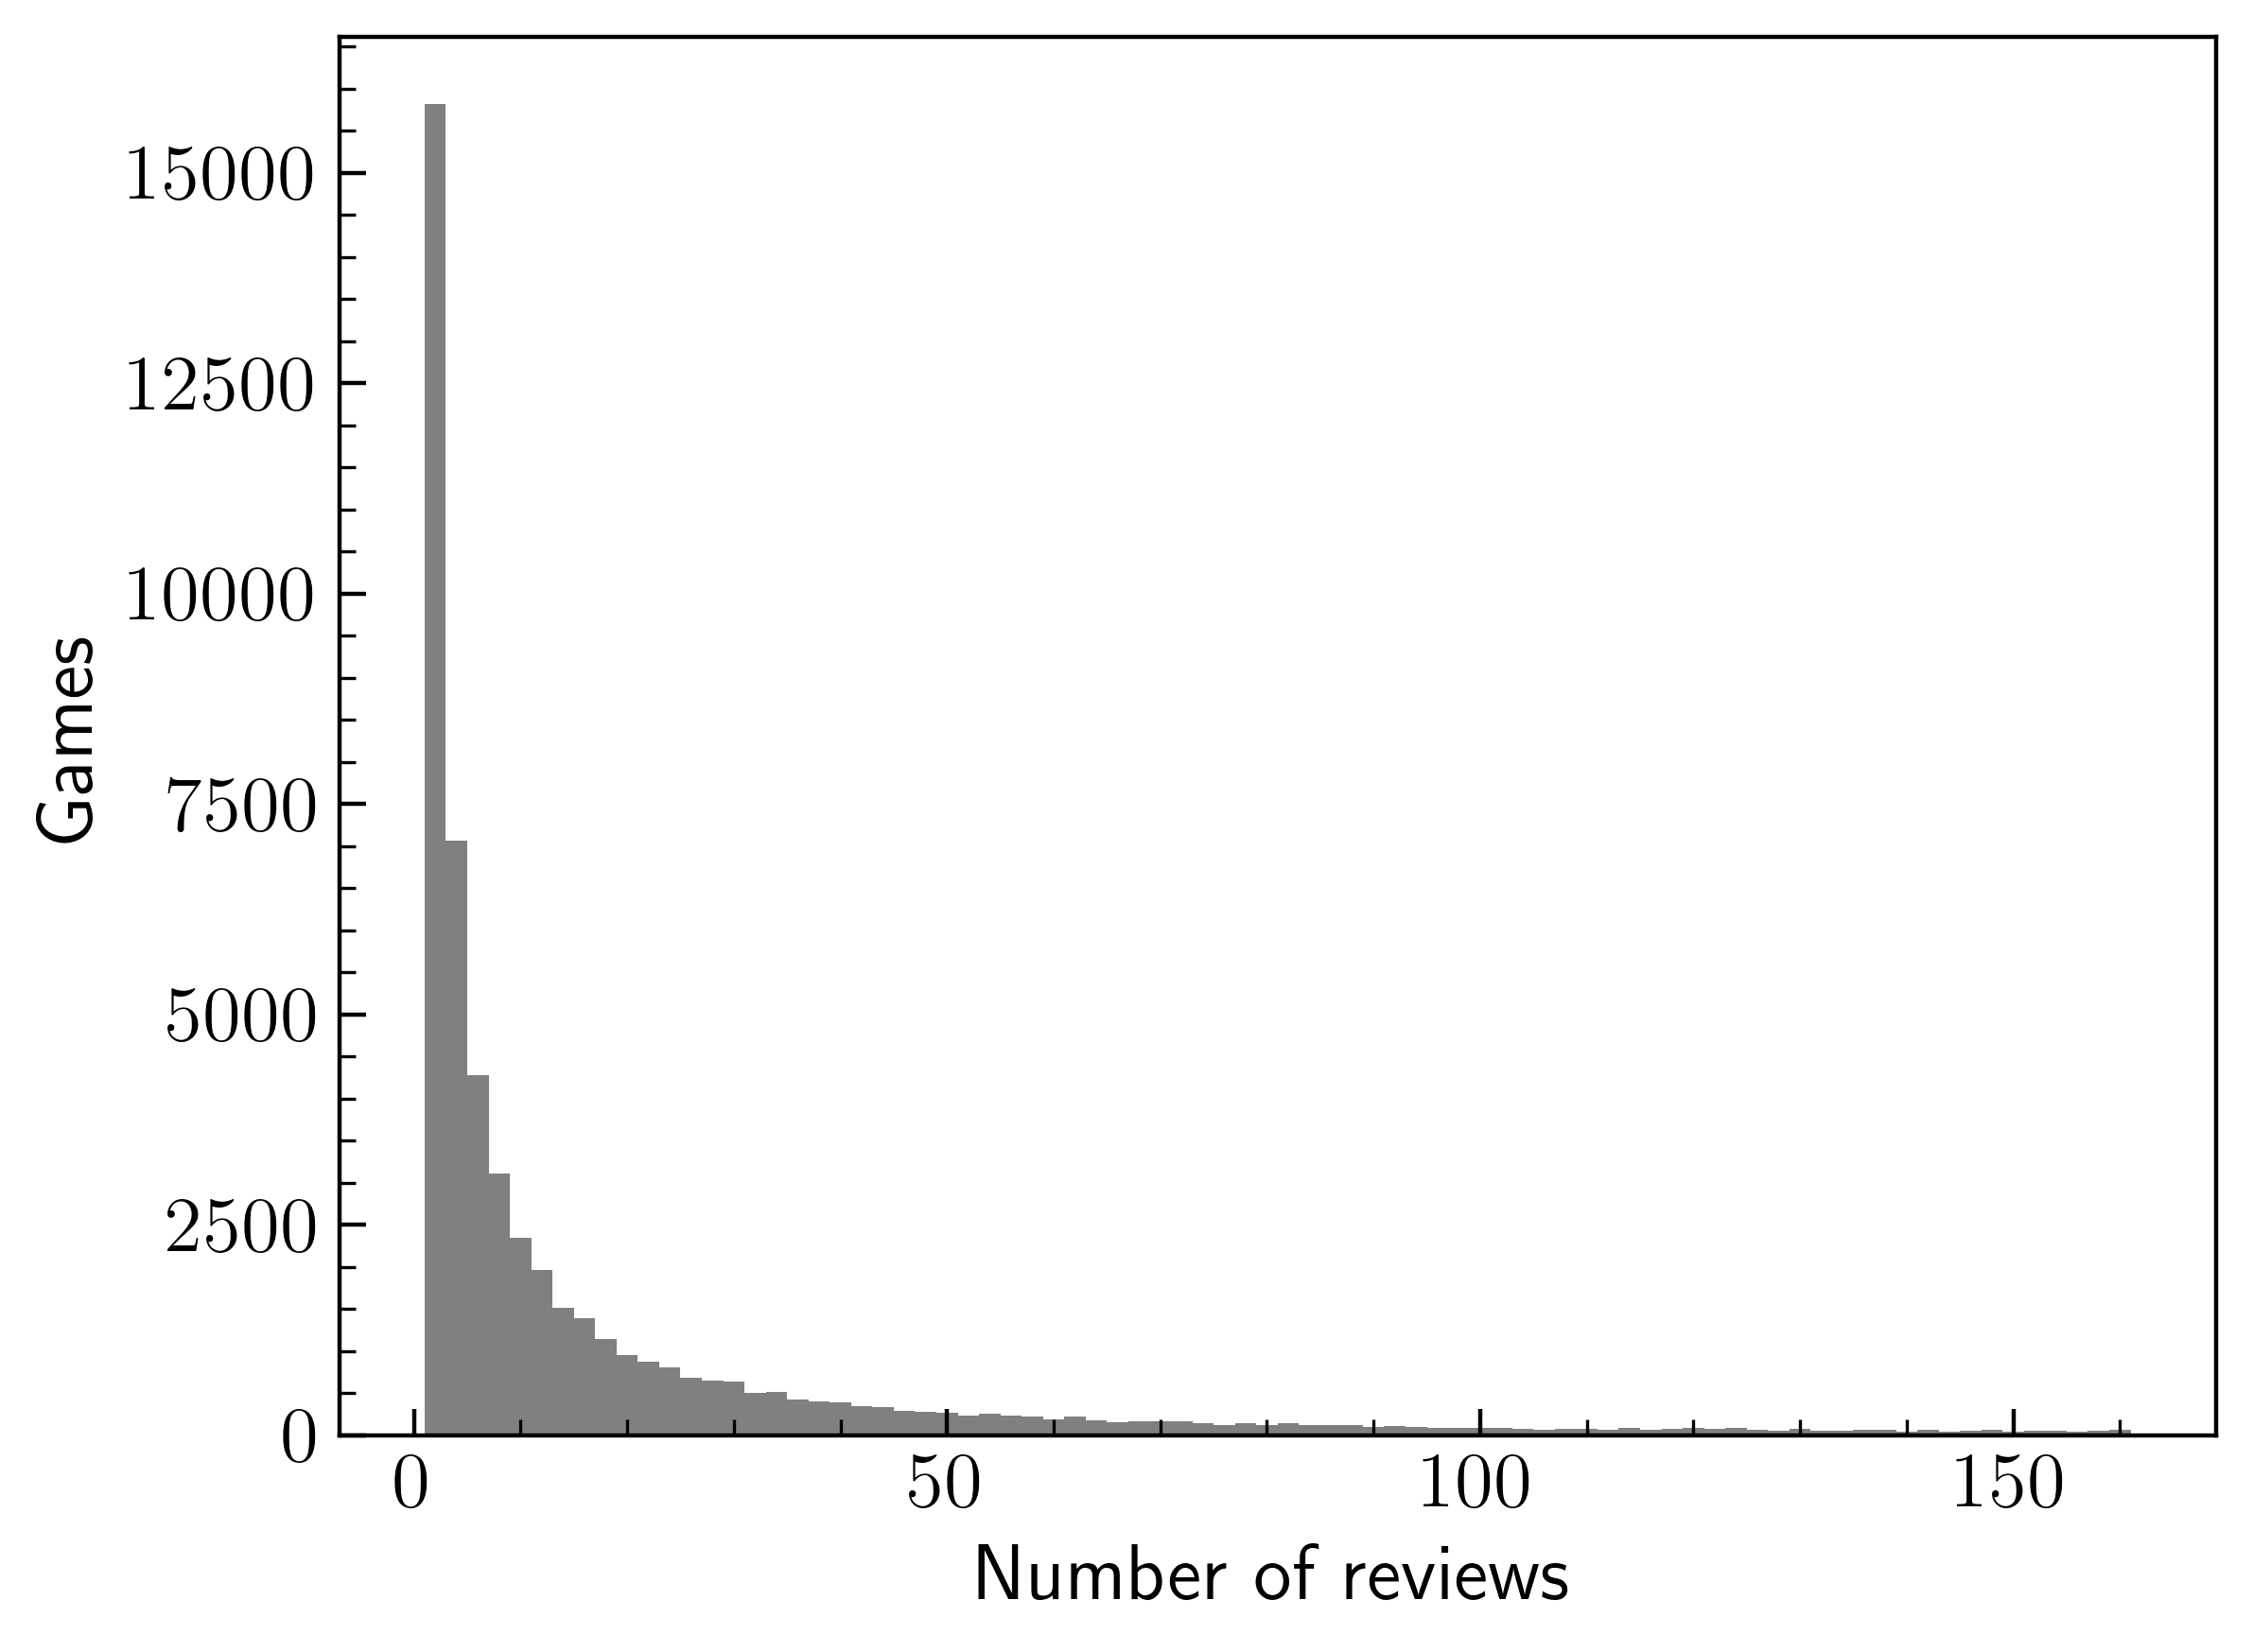
\includegraphics[width=\textwidth]{figures/03_dataset/05_hist_game_reviews.png}
        \caption{Number of reviews left for games.}
        \label{fig:Dataset_HistGameReviews}
    \end{subfigure}
    \caption{Review count distributions.}
    \label{fig:Dataset_HistsReviews}
\end{figure}

\subsection{Polarities}

The distribution of users based on the proportion of their reviews that are positive can be seen in Figure \ref{fig:Dataset_HistsPolarities}. When all users are considered, the mean positive proportion is 88.5\% (\textit{SD} = 25.2\%) and the median is 100\%. When only users who have written at least five reviews are considered, the mean positive proportion is 85.8\% (\textit{SD} = 16.5\%) and the median is 90\%.

When all users are considered the vast majority of users have a positive proportion of 100\%. The distribution becomes a little more balanced when only users with five or more reviews are considered although it still skews strongly to the right.

\begin{figure}[ht]
    \centering
    \begin{subfigure}[ht]{0.49\textwidth}
        \centering
        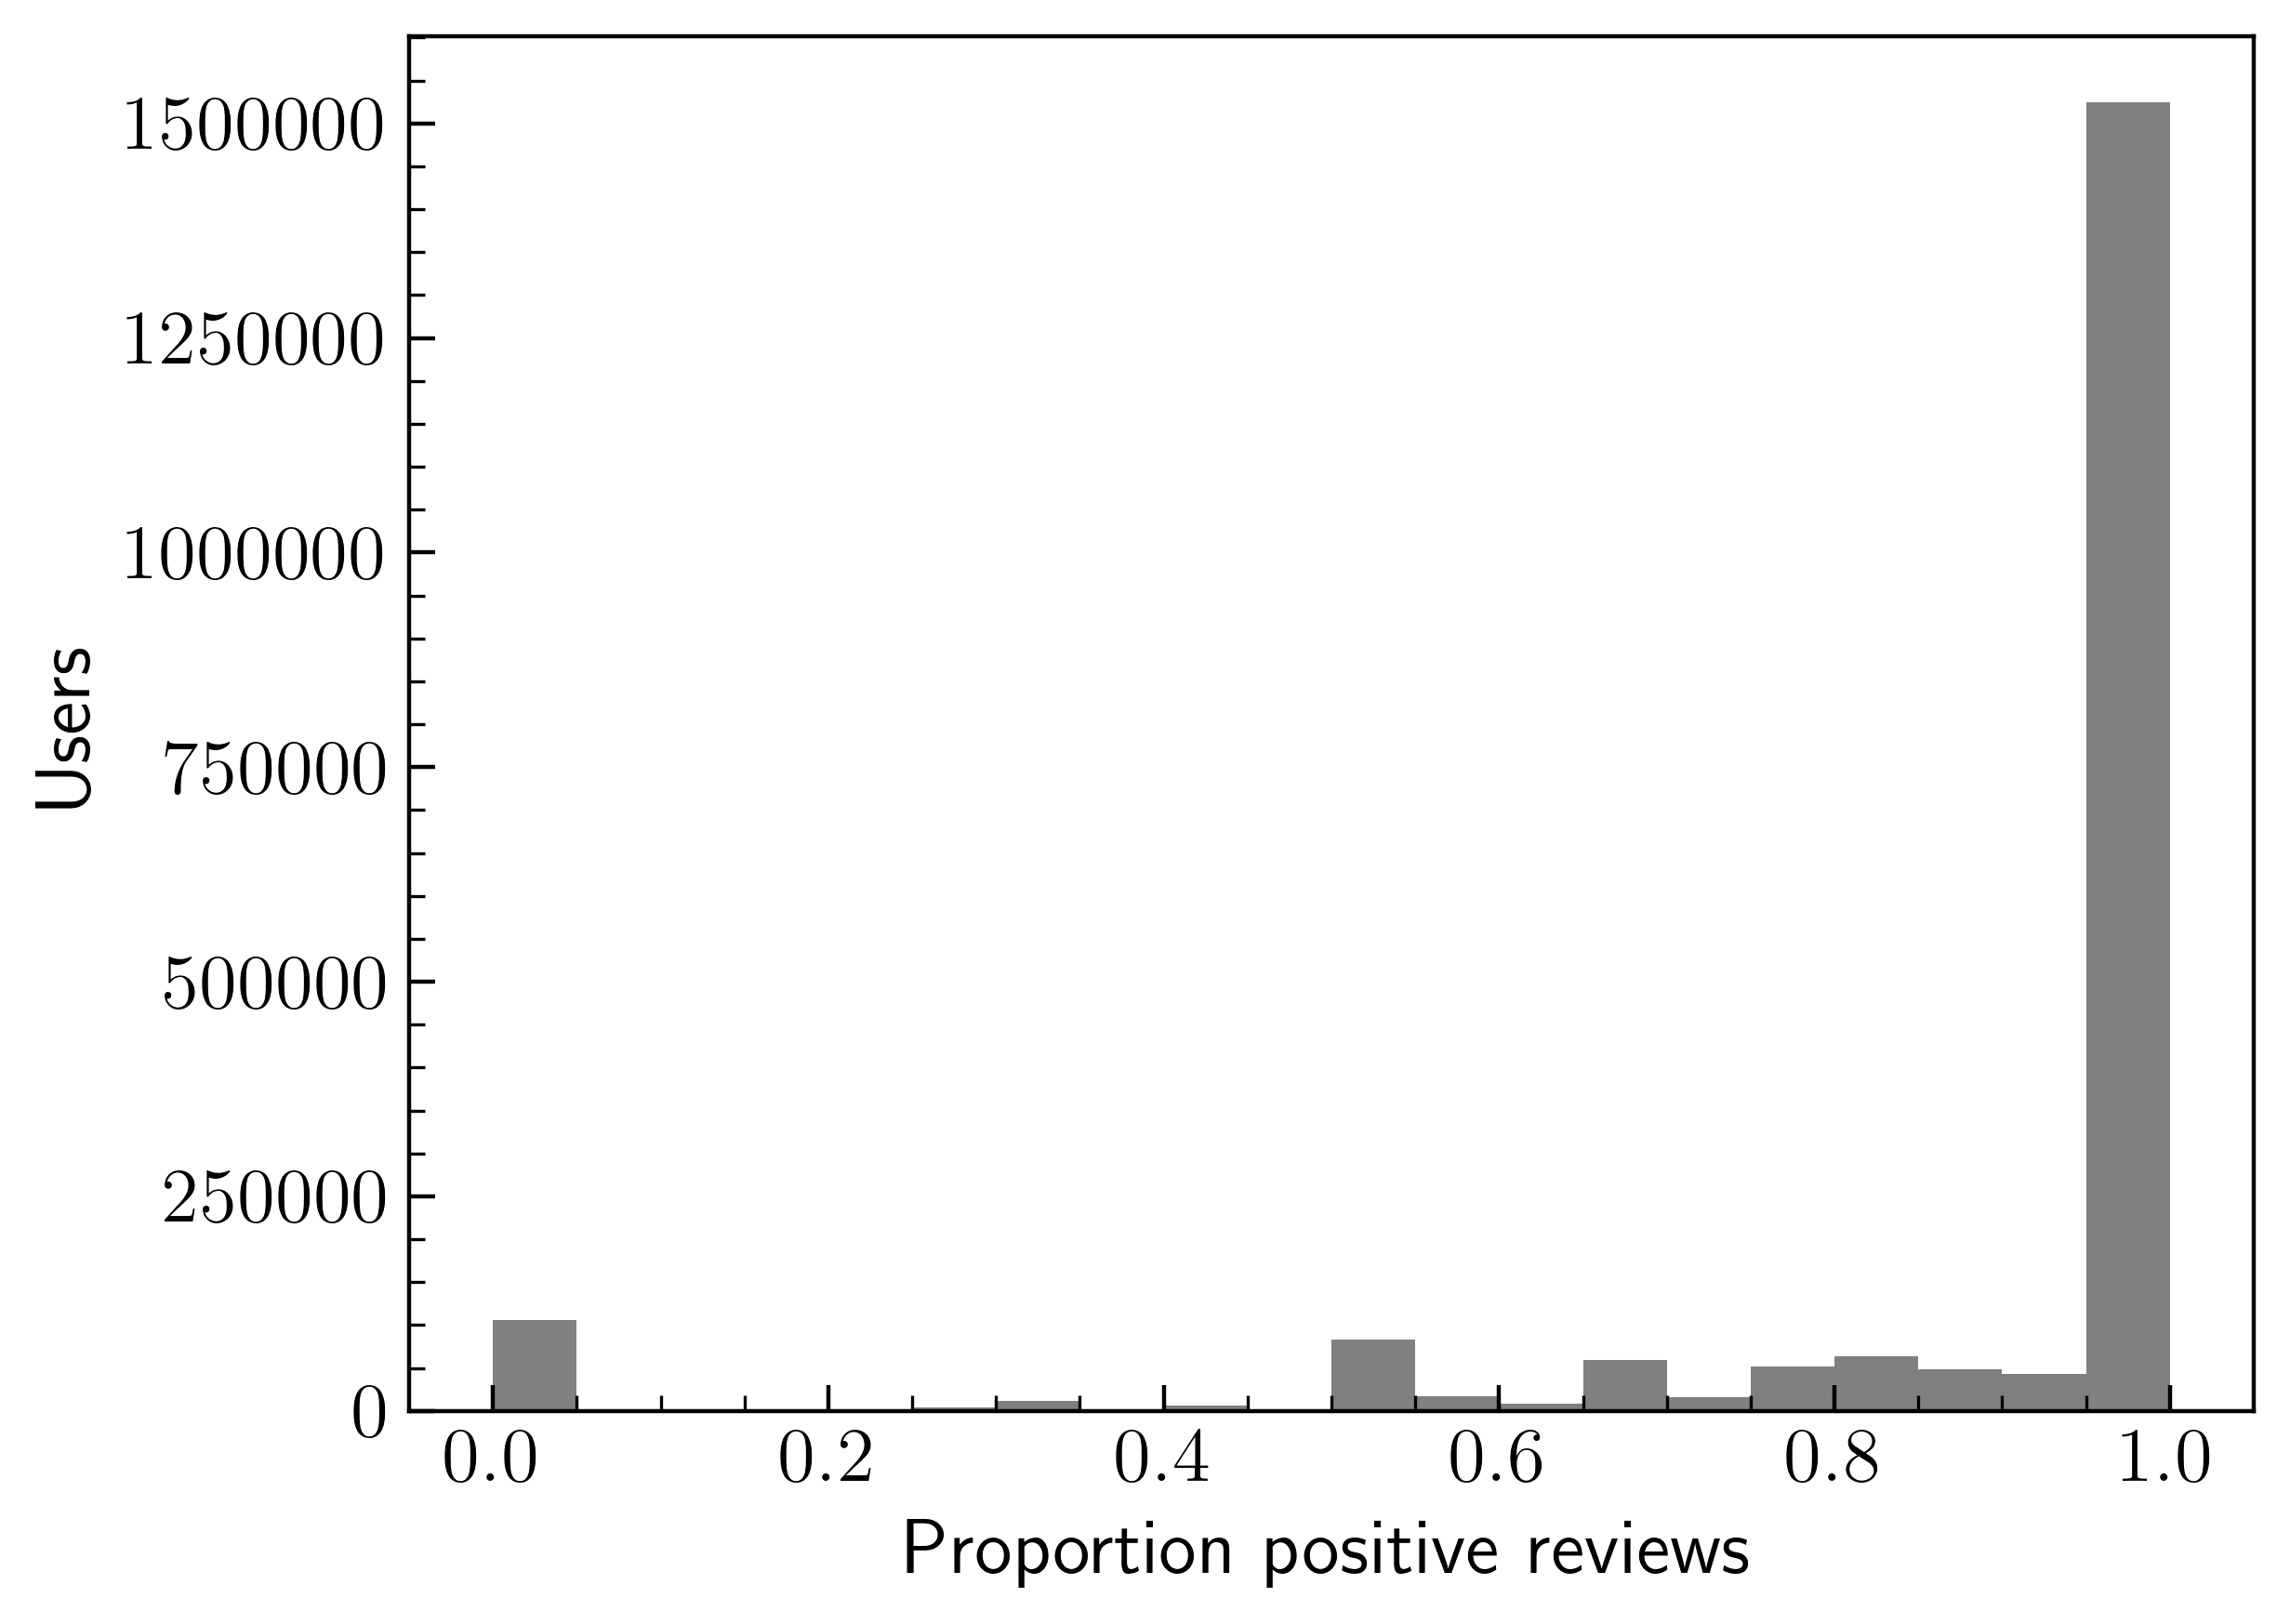
\includegraphics[width=\textwidth]{figures/03_dataset/06_hist_user_polarities_min1.png}
        \caption{All users.}
        \label{fig:Dataset_HistPolaritiesMin1}
    \end{subfigure}
    \hfill
    \begin{subfigure}[ht]{0.49\textwidth}
        \centering
        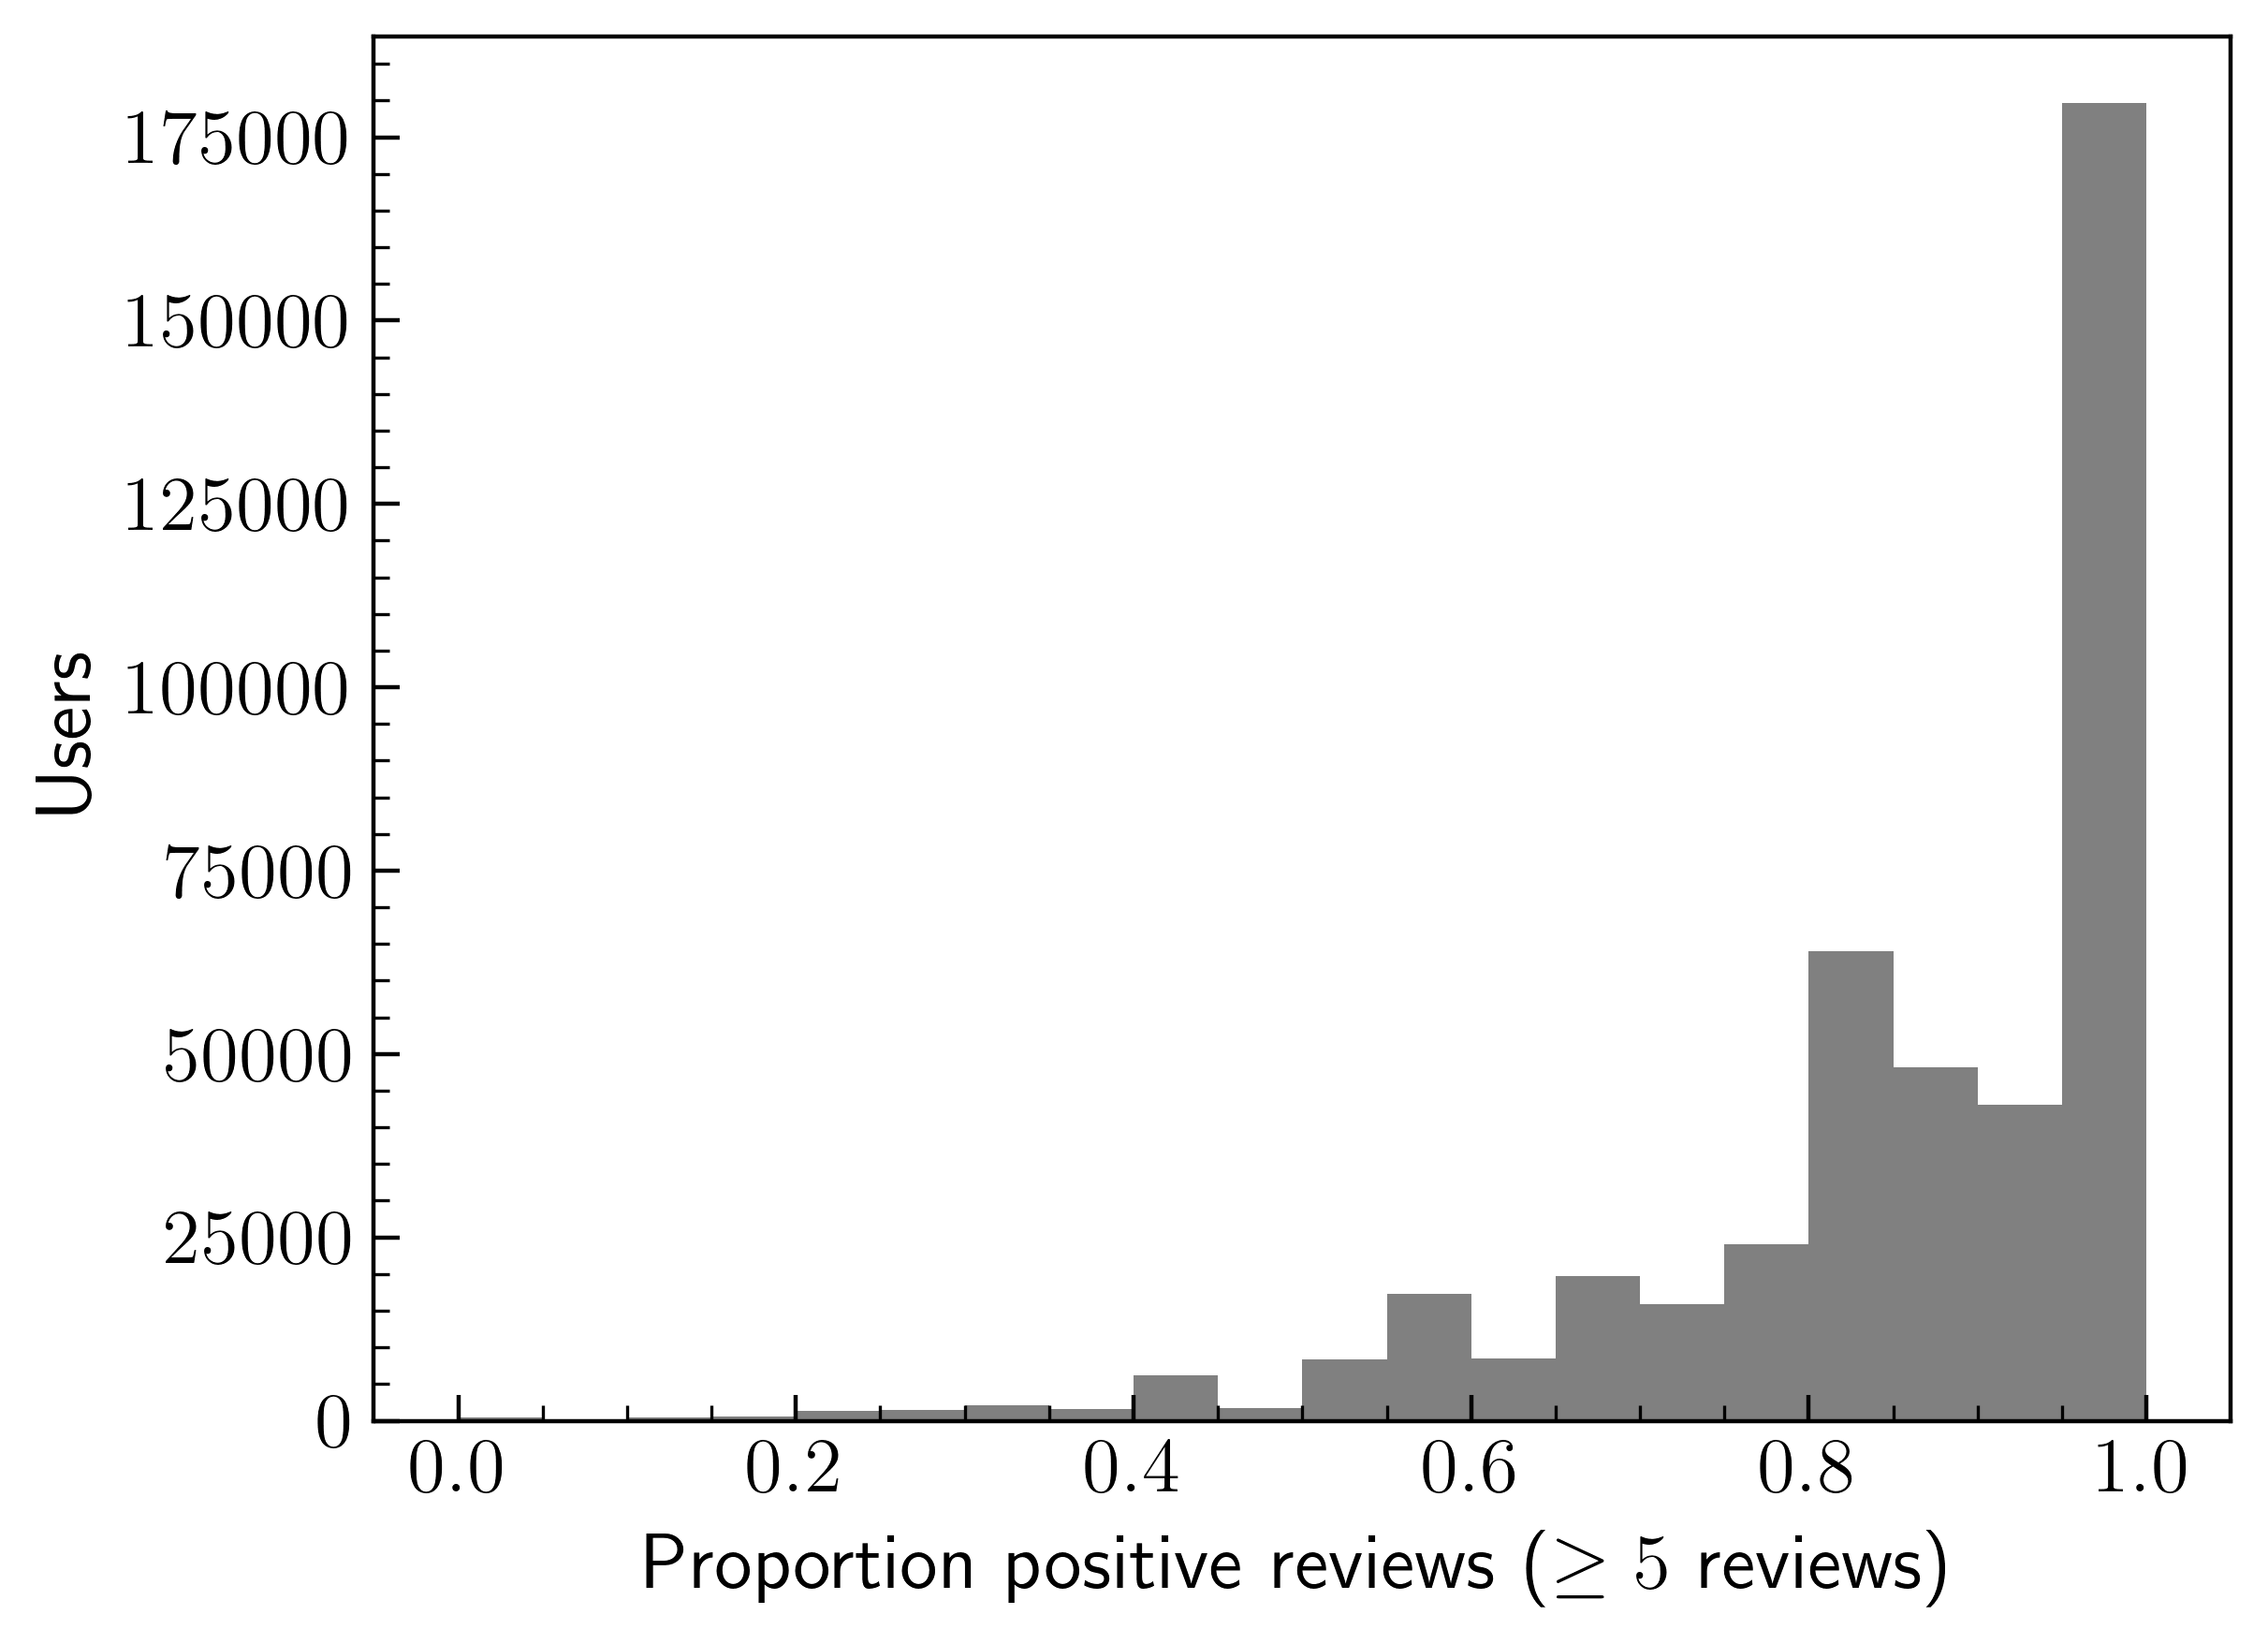
\includegraphics[width=\textwidth]{figures/03_dataset/07_hist_user_polarities_min5.png}
        \caption{Users with at least five reviews.}
        \label{fig:Dataset_HistPolaritiesMin5}
    \end{subfigure}
    \caption{Proportion of users' reviews that are positive.}
    \label{fig:Dataset_HistsPolarities}
\end{figure}

\subsection{Miscellaneous Features}

The distribution of some review features can be seen in Figure \ref{fig:Dataset_BarsCounts}. Across the dataset, 85\% of reviews are positive, 9.6\% are for an early access game and 14.4\% were updated by the author at some point.

\begin{figure}[ht]
    \centering
    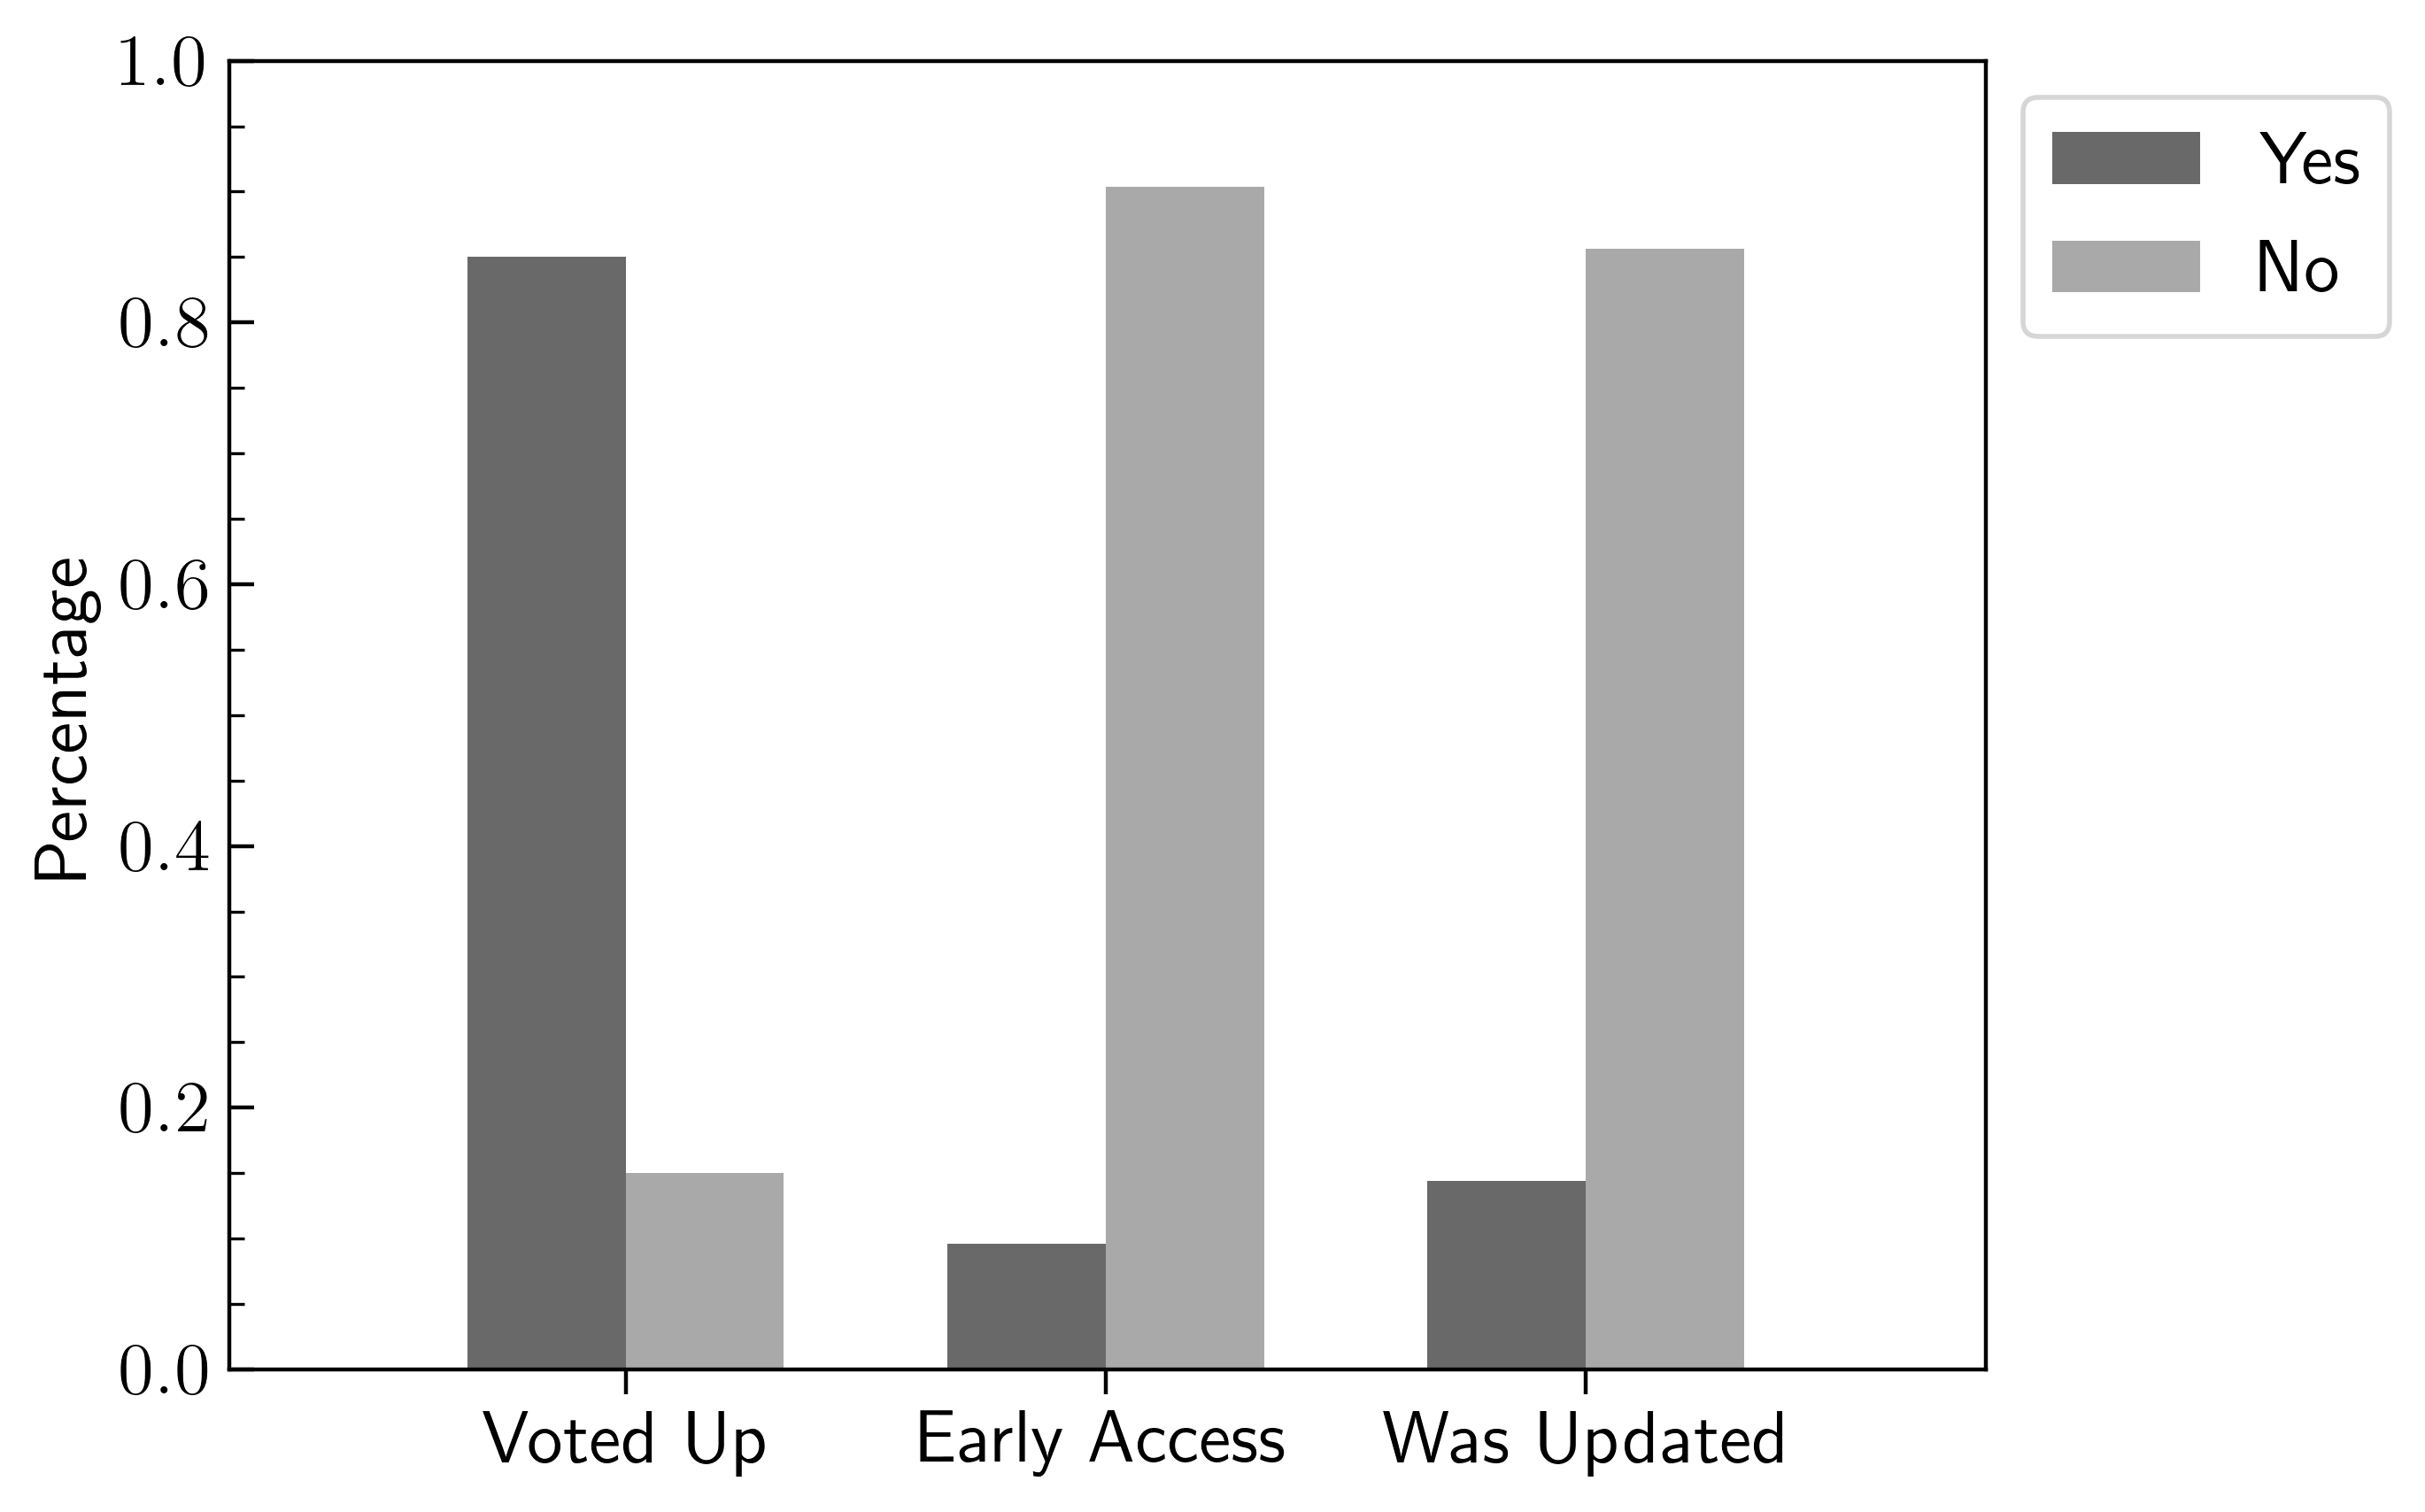
\includegraphics[scale=0.55]{figures/03_dataset/08_bars_counts.png}
    \caption{Percentage of reviews that were positive (voted up), early access and updated.}
    \label{fig:Dataset_BarsCounts}
\end{figure}

\subsection{Timestamps}

The years in which reviews were written can be seen in Figure \ref{fig:Dataset_BarsTimestamps}.

\begin{figure}[ht]
    \centering
    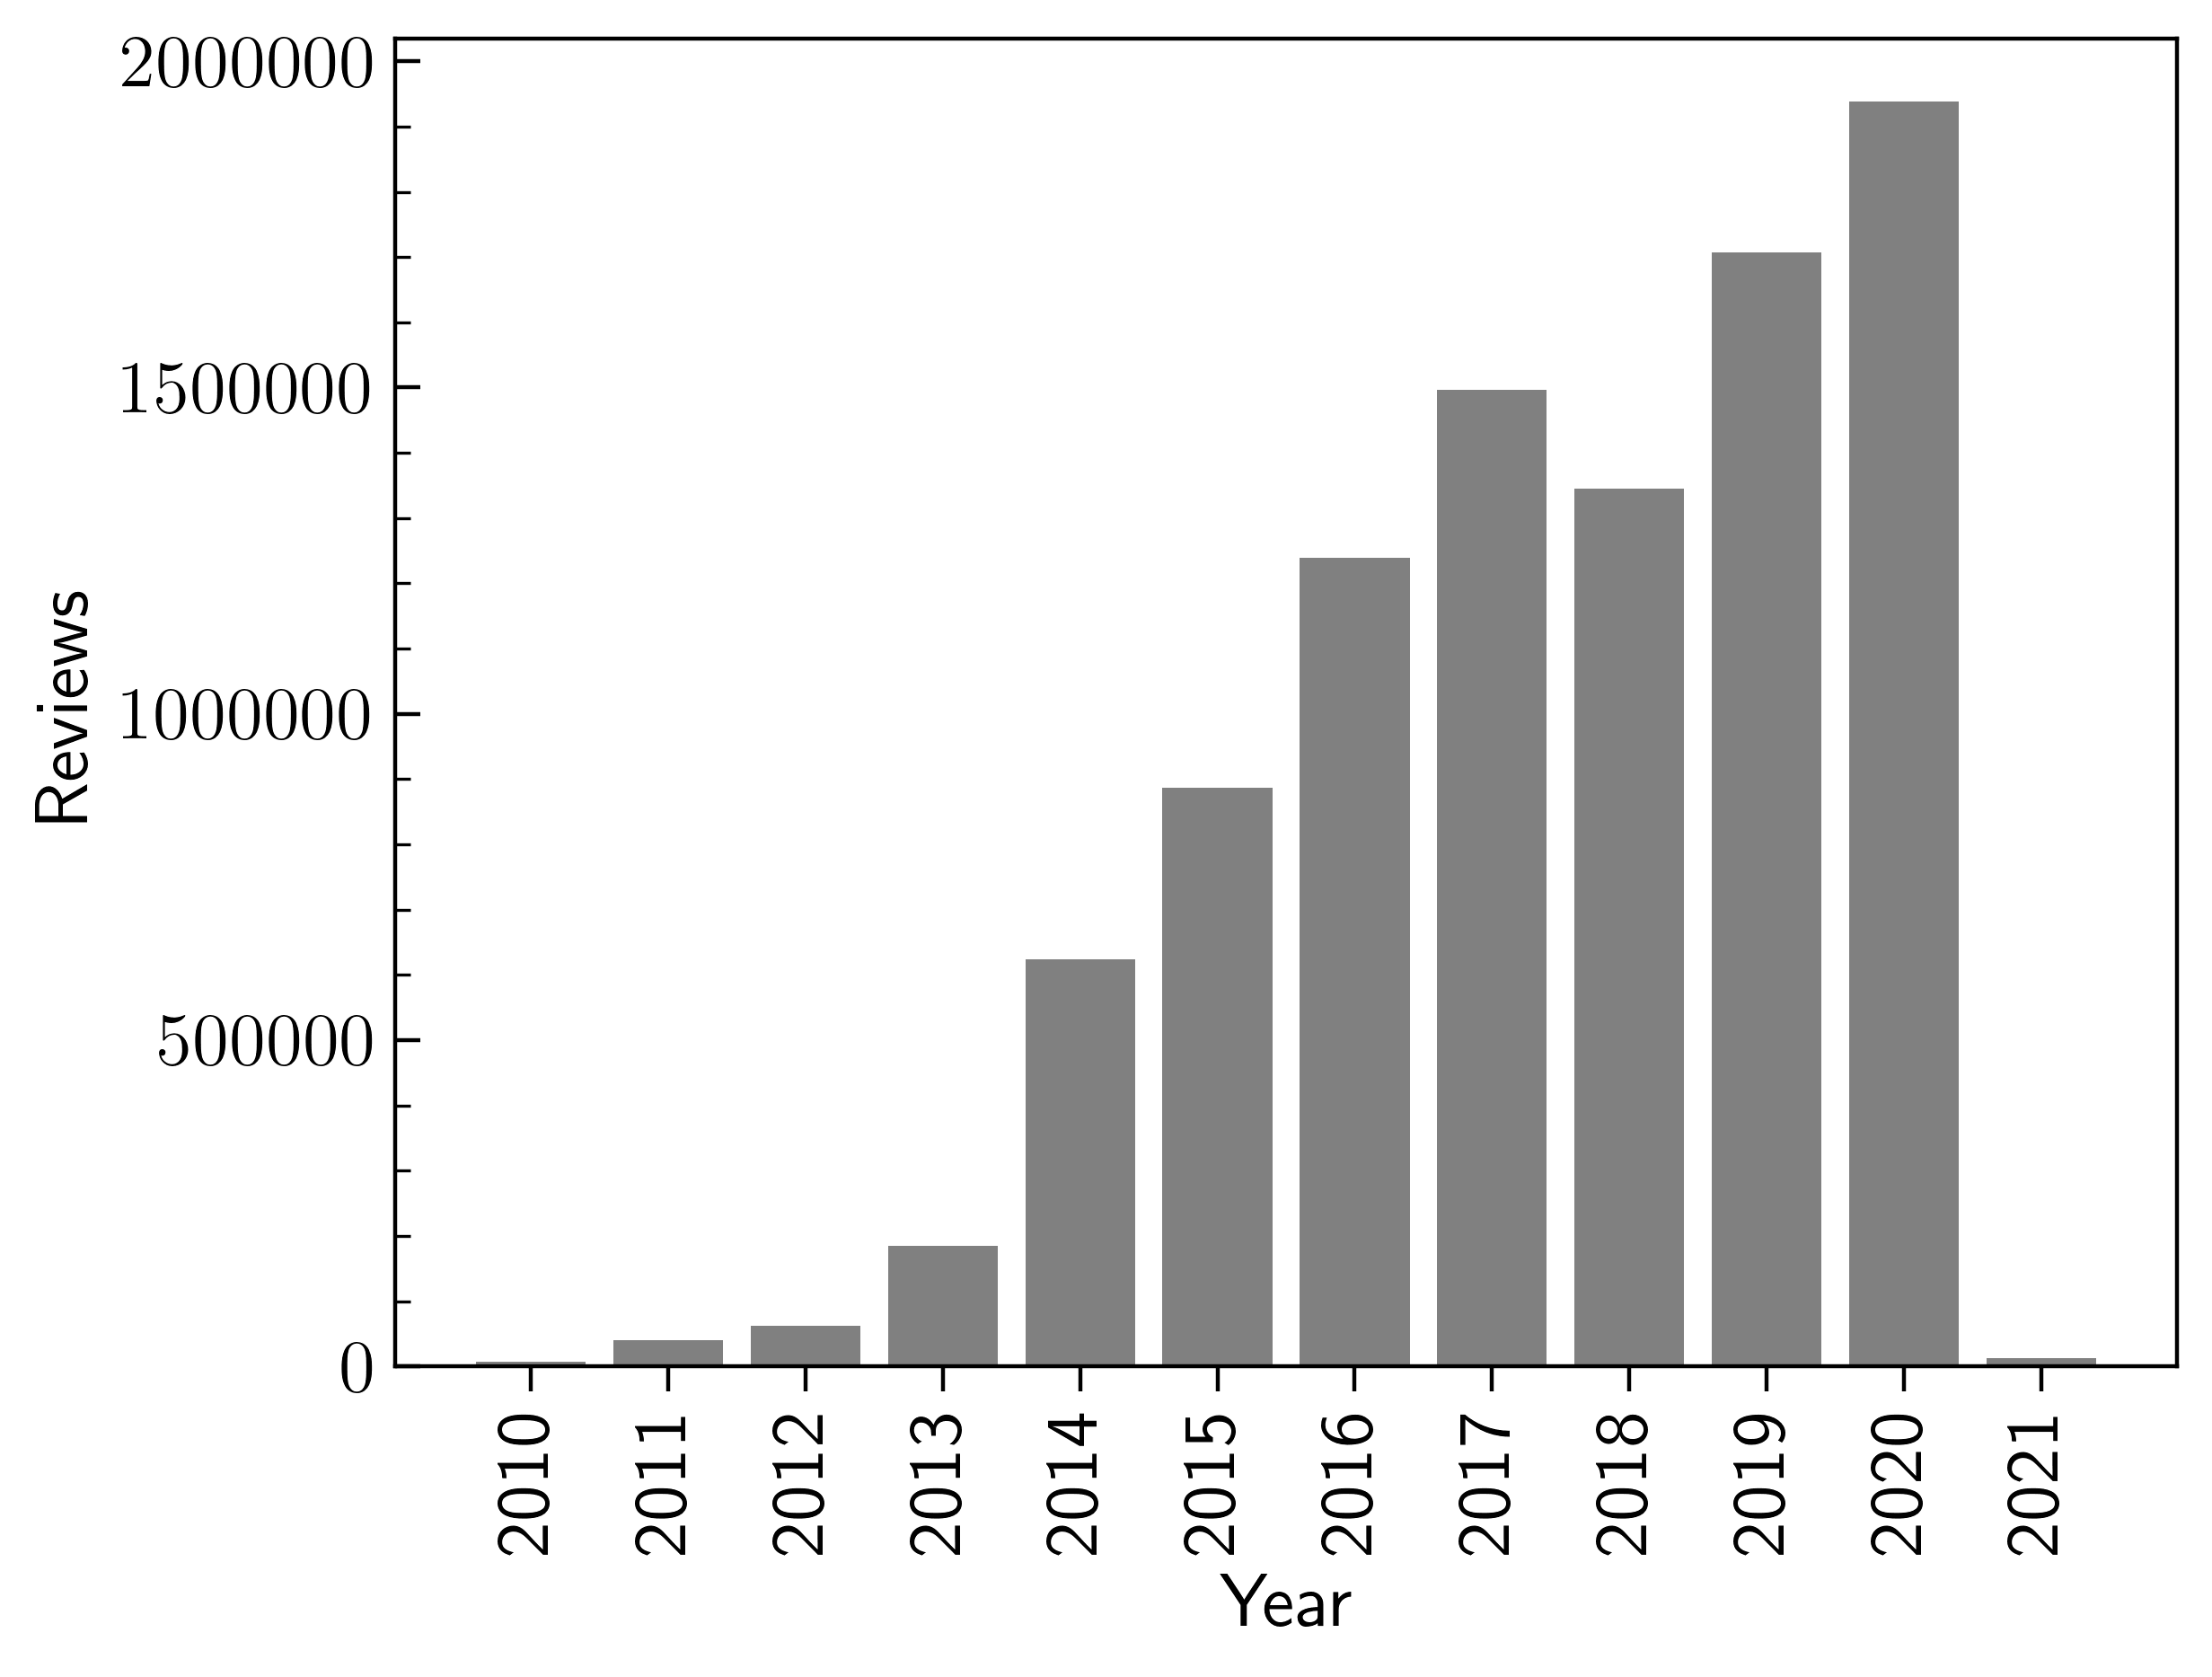
\includegraphics[scale=0.55]{figures/03_dataset/09_bars_review_dates.png}
    \caption{Years in which reviews were written.}
    \label{fig:Dataset_BarsTimestamps}
\end{figure}

\subsection{Playtime}

The amount of hours that users played the games they reviewed (in total) can be seen in Figure \ref{fig:Dataset_HistPlaytimes}. Reviews where the user played the game for over 152.4 hours, 16.4\% of all reviews, have been excluded from the histogram. The mean amount of hours users played the games they reviewed is 159.1 (\textit{SD} = 540.6) and the median is 12.2. 25\% of users played the game they reviewed for 2.9 hours or less and 75\% of users played the game they reviewed for 62.7 hours or less.

\begin{figure}[ht]
    \centering
    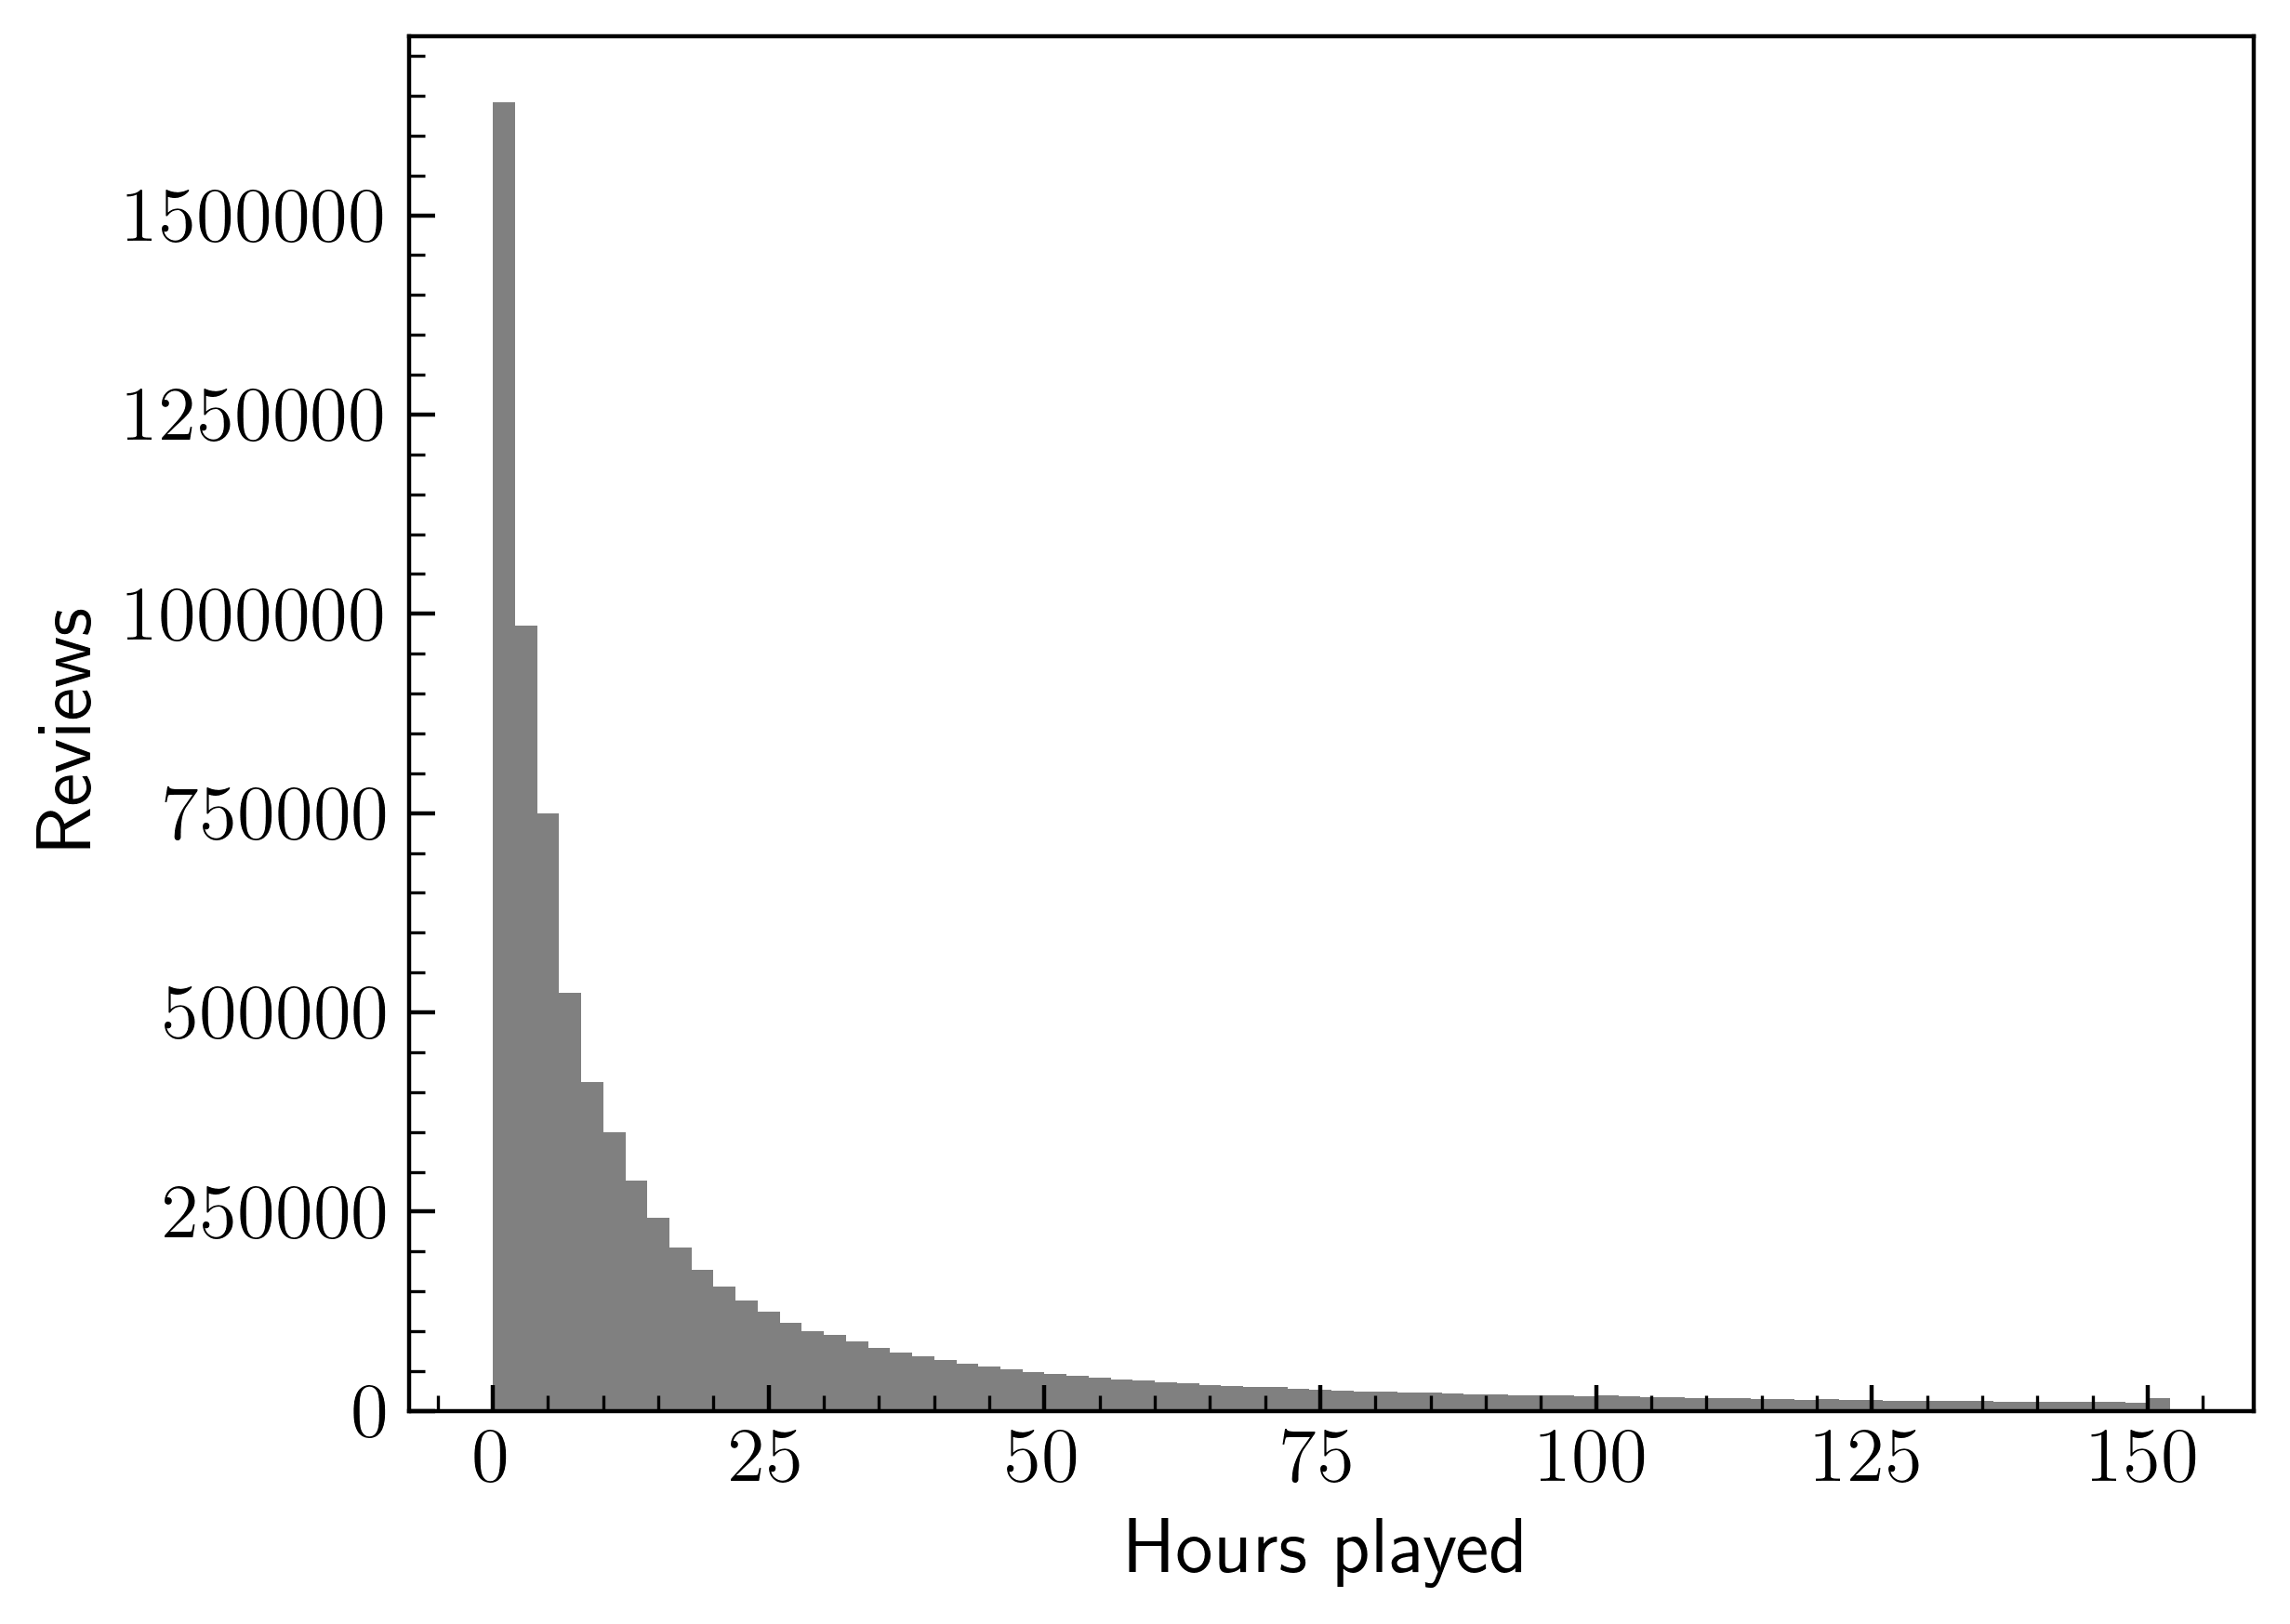
\includegraphics[scale=0.55]{figures/03_dataset/10_hist_review_playtimes.png}
    \caption{Number of hours that reviewed games were played (in total).}
    \label{fig:Dataset_HistPlaytimes}
\end{figure}

\subsection{Votes}

The number of votes up that reviews received can be seen in Figure \ref{fig:Dataset_HistVotes}. Reviews with more than 17 votes, 4.5\% of all reviews, have been excluded from the histogram. The mean number of votes reviews received is 4.3 (\textit{SD} = 22.9) and the median is 0. A majority of reviews didn't receive a single vote and 75\% of reviews received 2 votes or fewer.

\begin{figure}[ht]
    \centering
    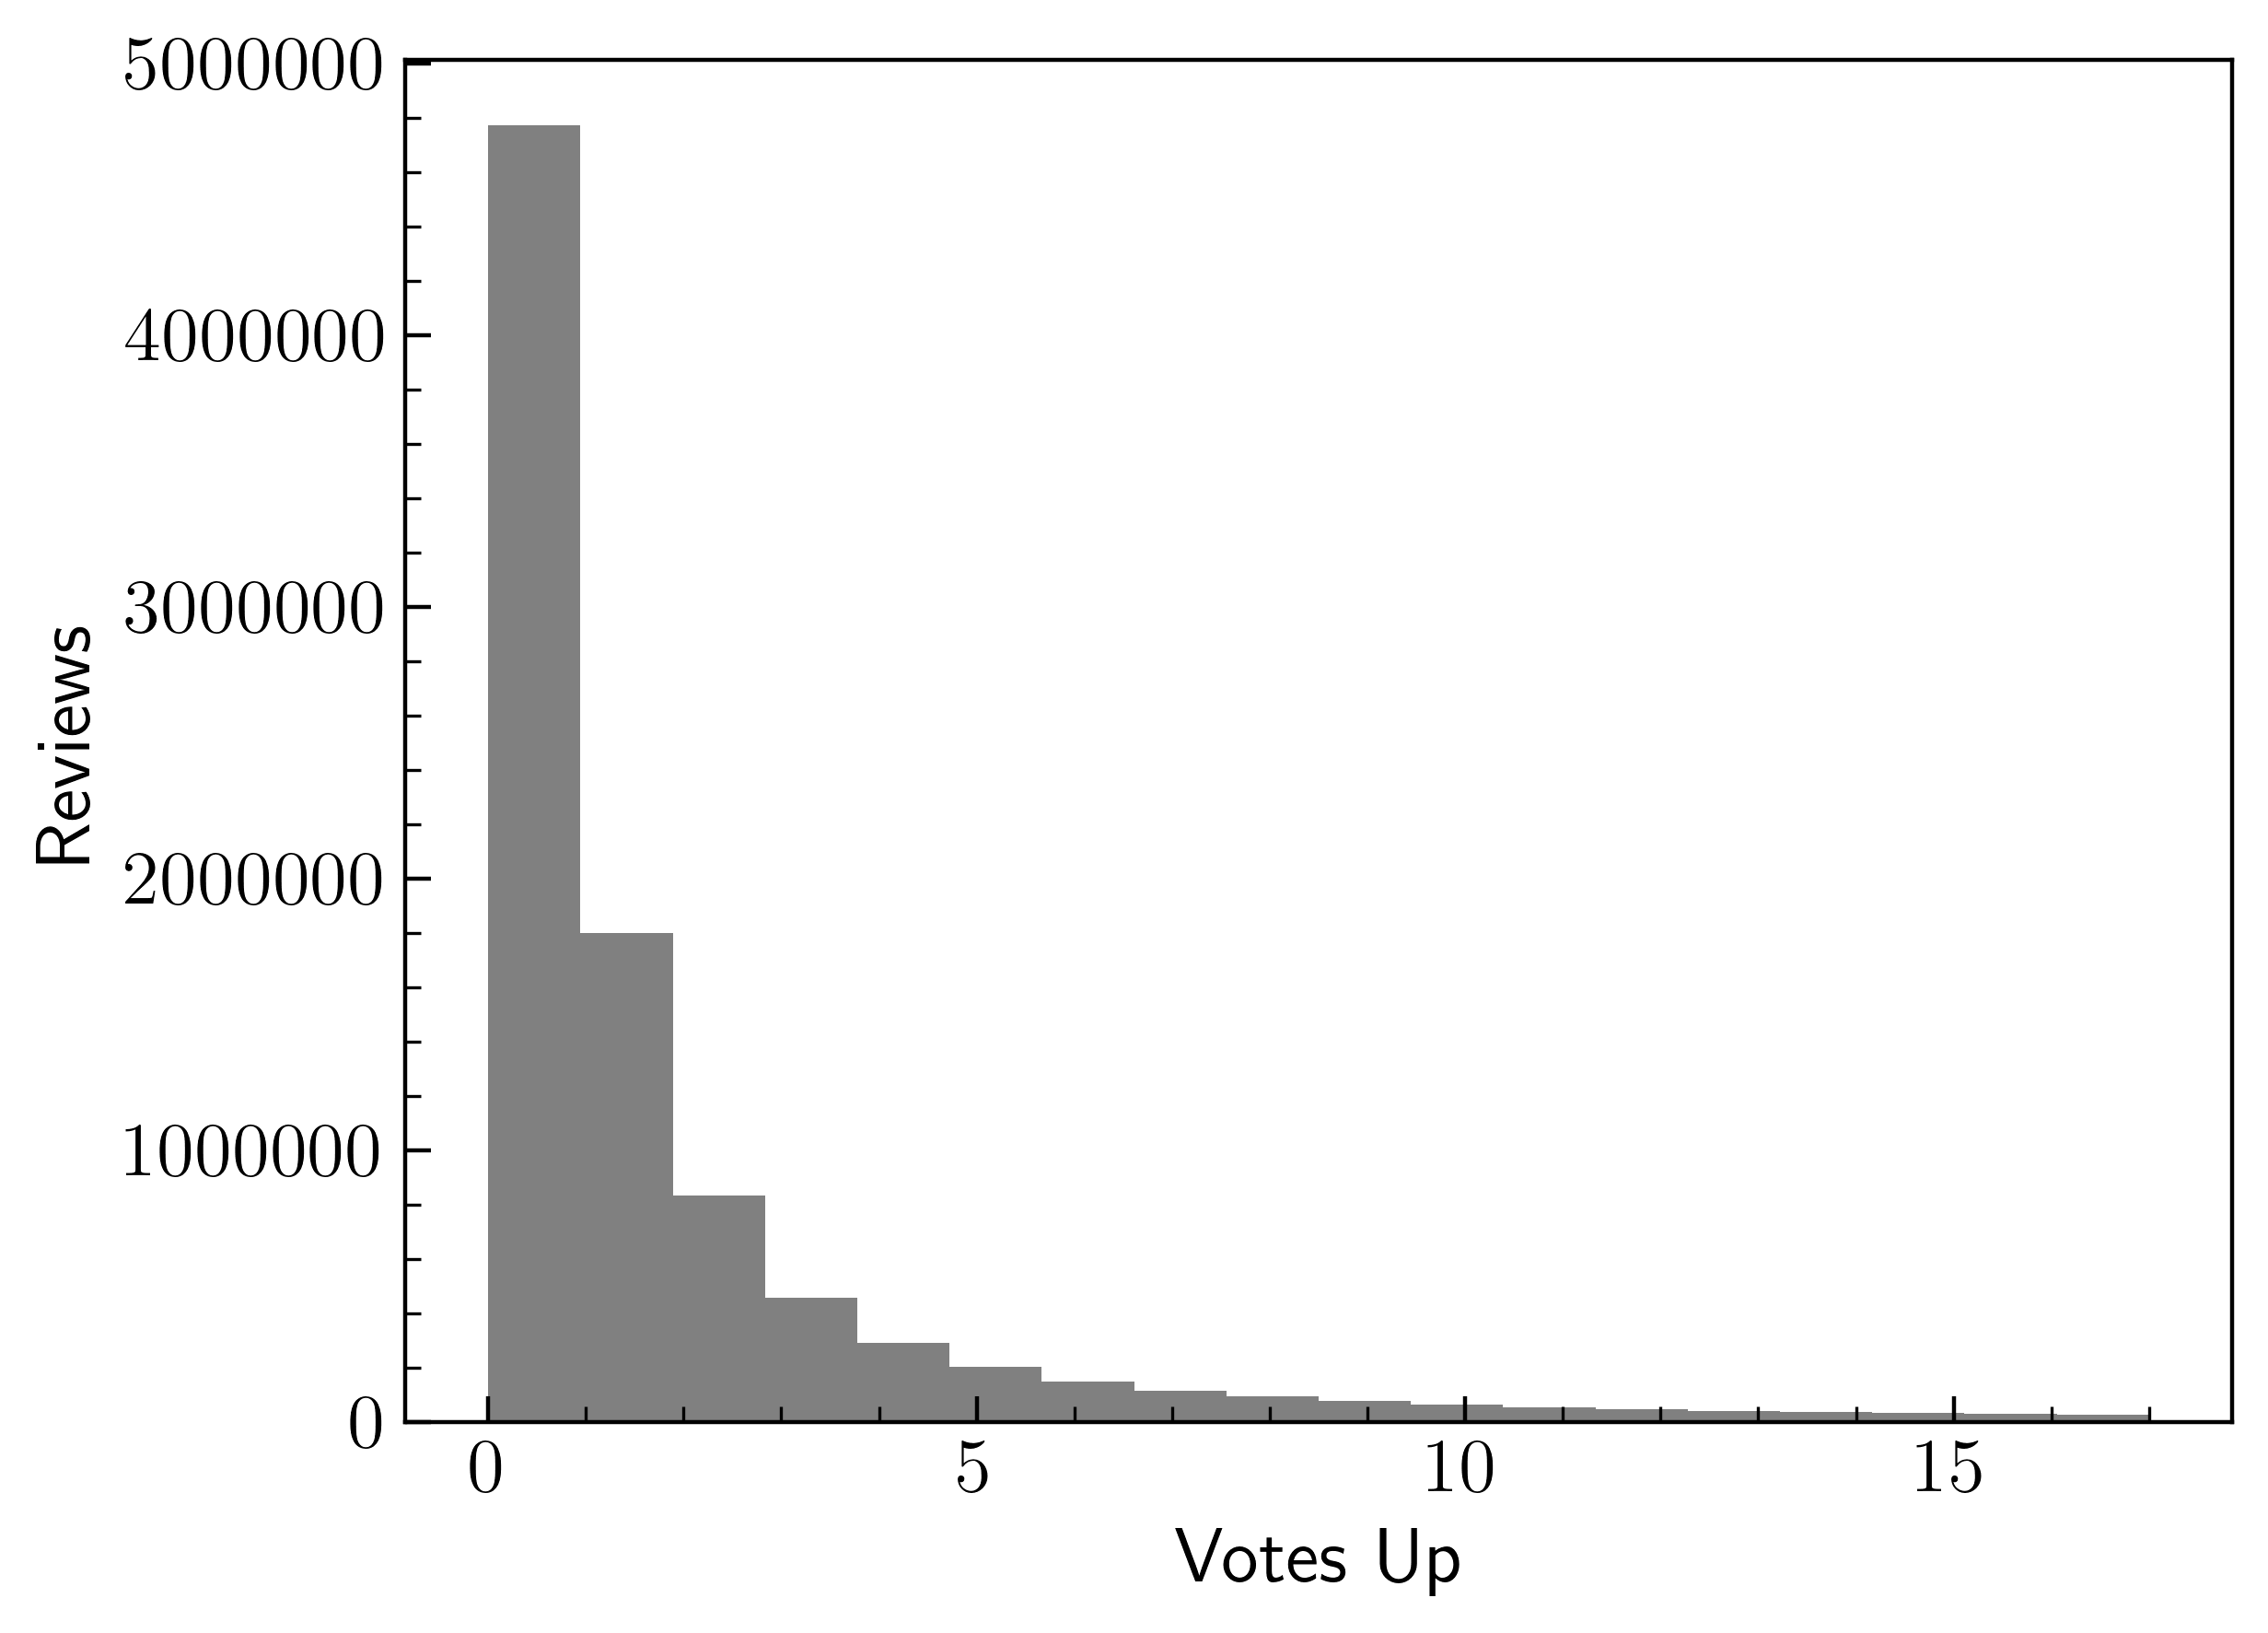
\includegraphics[scale=0.55]{figures/03_dataset/11_hist_review_votes.png}
    \caption{Number of votes up that reviews received.}
    \label{fig:Dataset_HistVotes}
\end{figure}

\section{Review Texts} \label{sec:Dataset_ReviewTexts}

The language each review was written in and the number of words each review contained was determined for nearly 70\% of all reviews in the dataset using the spaCy library in Python \cite{spacy}. Language detection is implemented using a Python port \cite{PyPi_LangDetect} of Google's language-detection library \cite{Nakatani2010_LangDetect} which supports over 50 languages.

\subsection{Languages}

The proportion of languages each review was written in can be seen in Figure \ref{fig:Dataset_BarsLangs}. Languages that less than 1\% of reviews are written in are excluded. Language proportions are shown for all reviews and for reviews with at least five words. When all reviews are considered the language detection algorithm fails to identify the language in approximately 3\% of reviews. When reviews with at least five words are considered this failure to identify the language occurs much less frequently and the proportion of reviews written in English increases to almost 50\%.

\begin{figure}[ht]
    \centering
    \begin{subfigure}[ht]{0.49\textwidth}
        \centering
        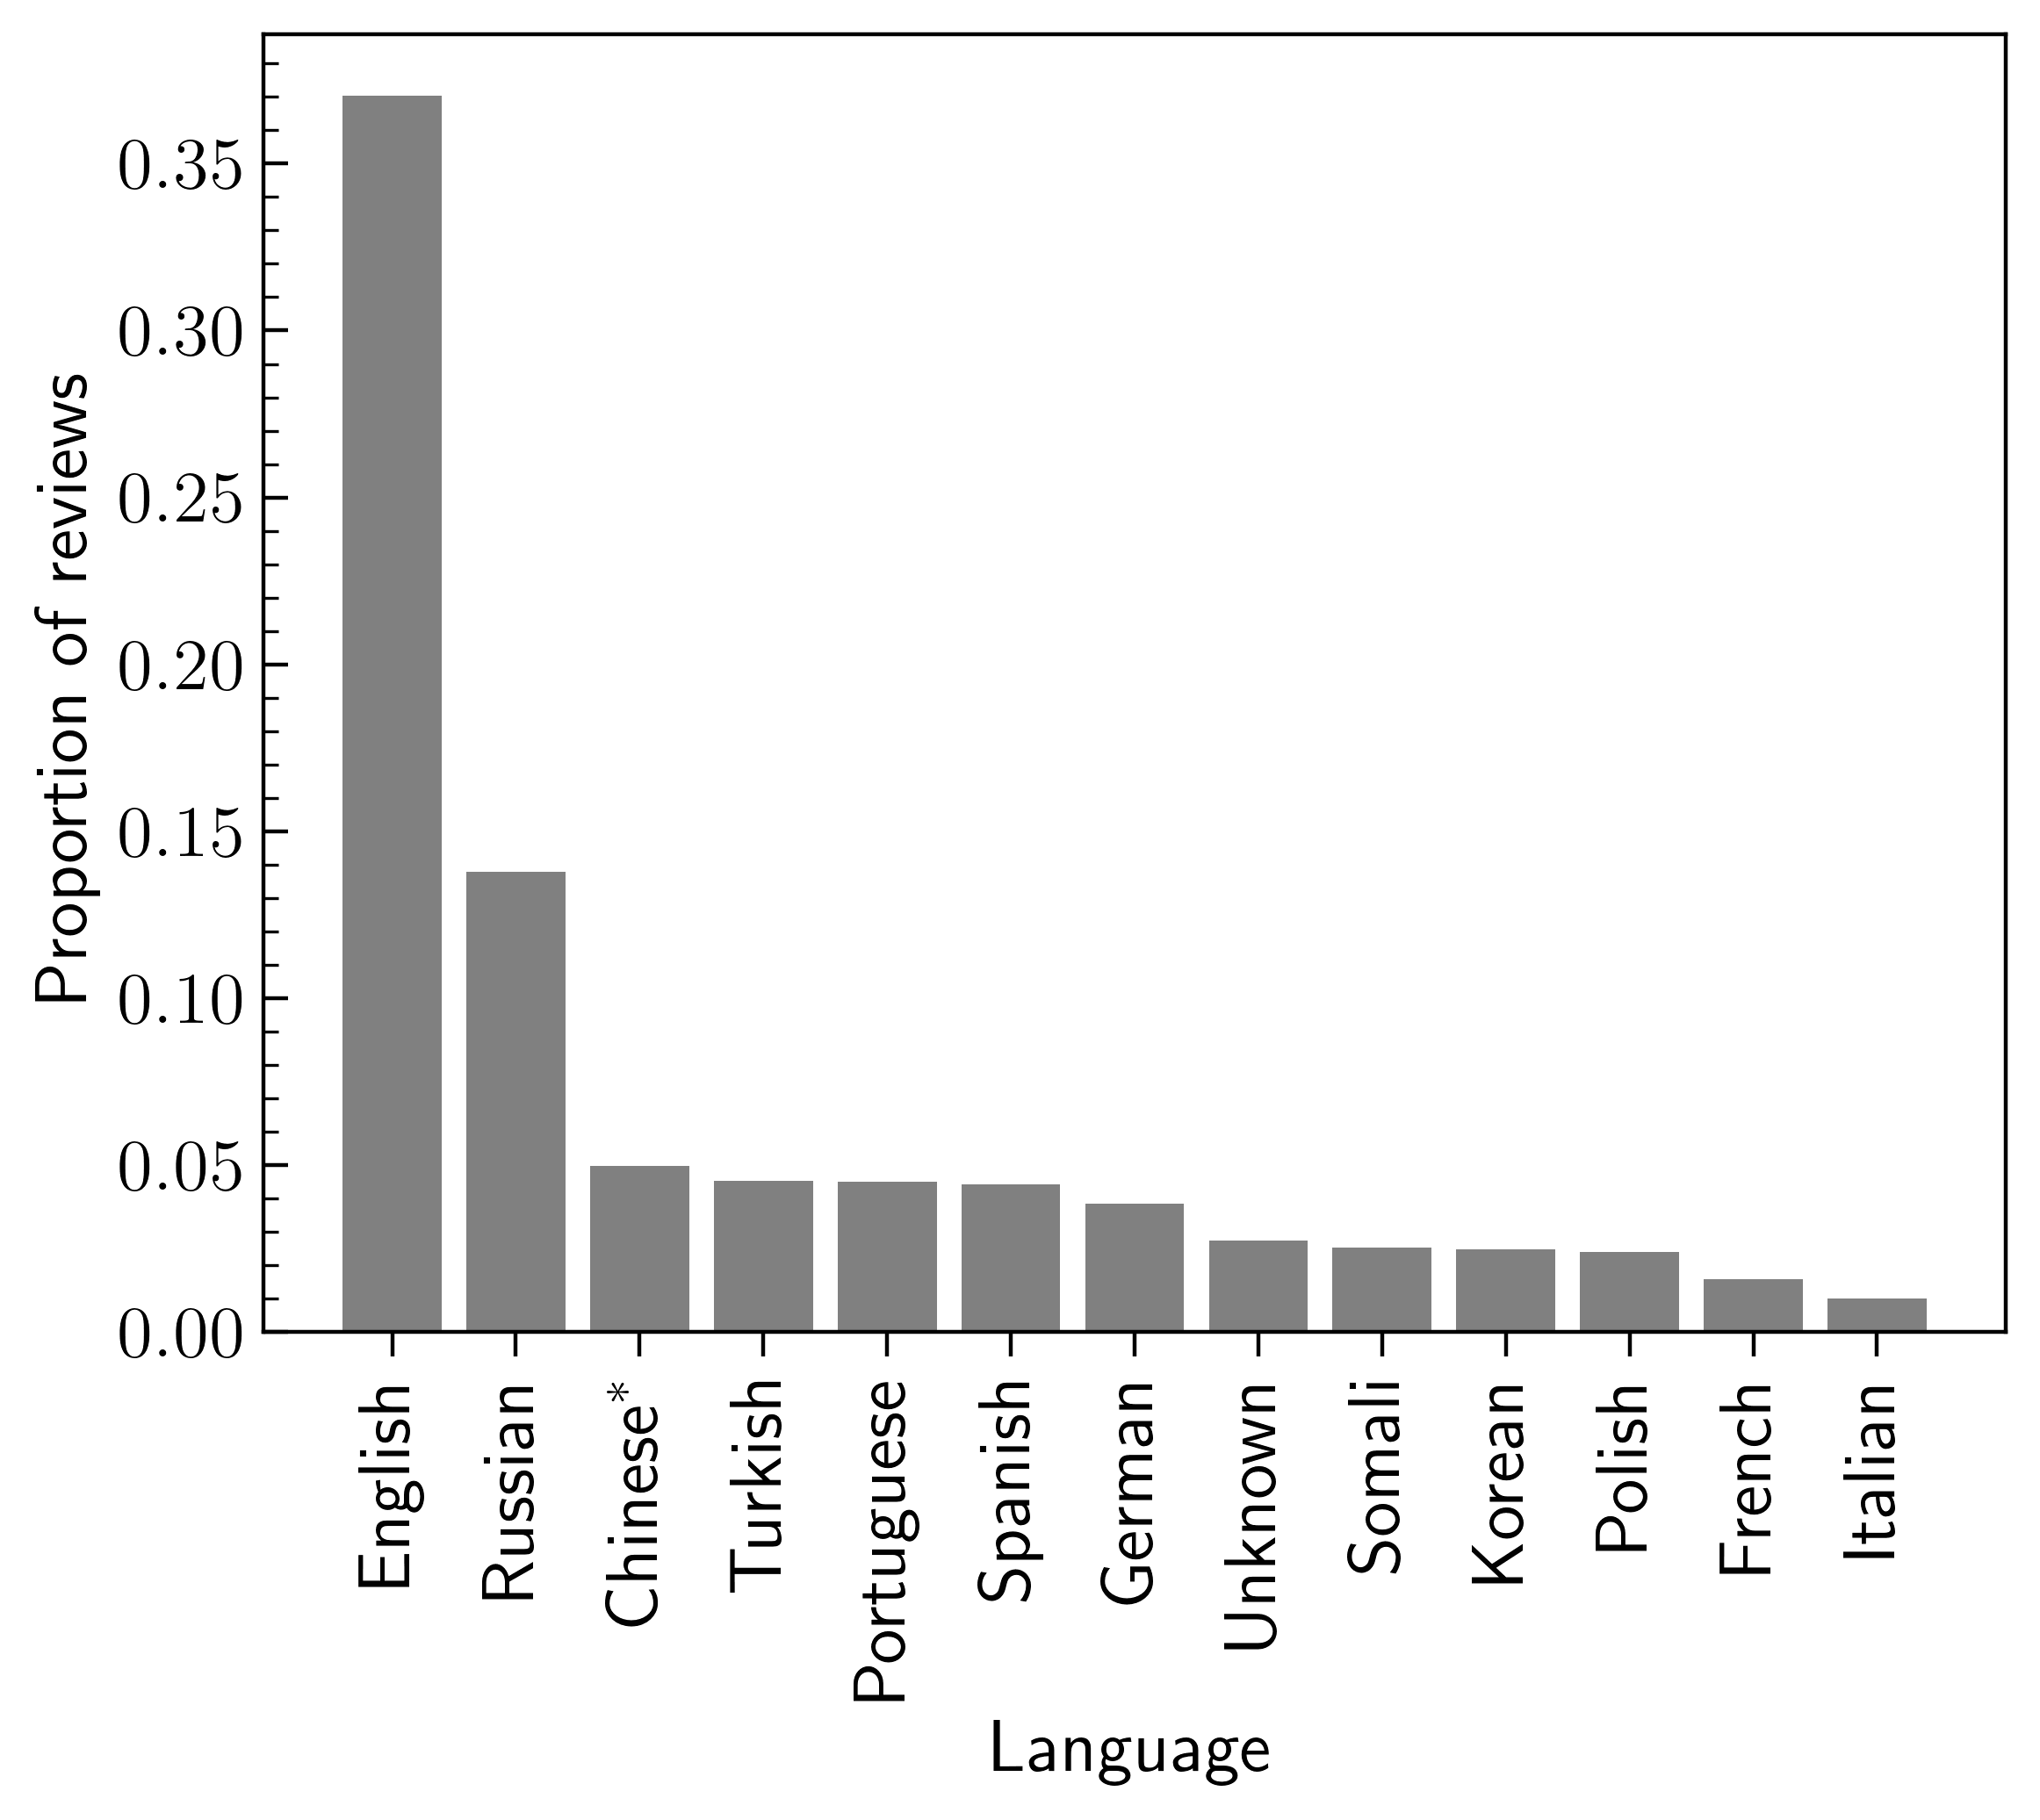
\includegraphics[width=\textwidth]{figures/03_dataset/12_bars_review_langs_min0.png}
        \caption{All reviews.}
        \label{fig:Dataset_BarsLangsMin1}
    \end{subfigure}
    \hfill
    \begin{subfigure}[ht]{0.49\textwidth}
        \centering
        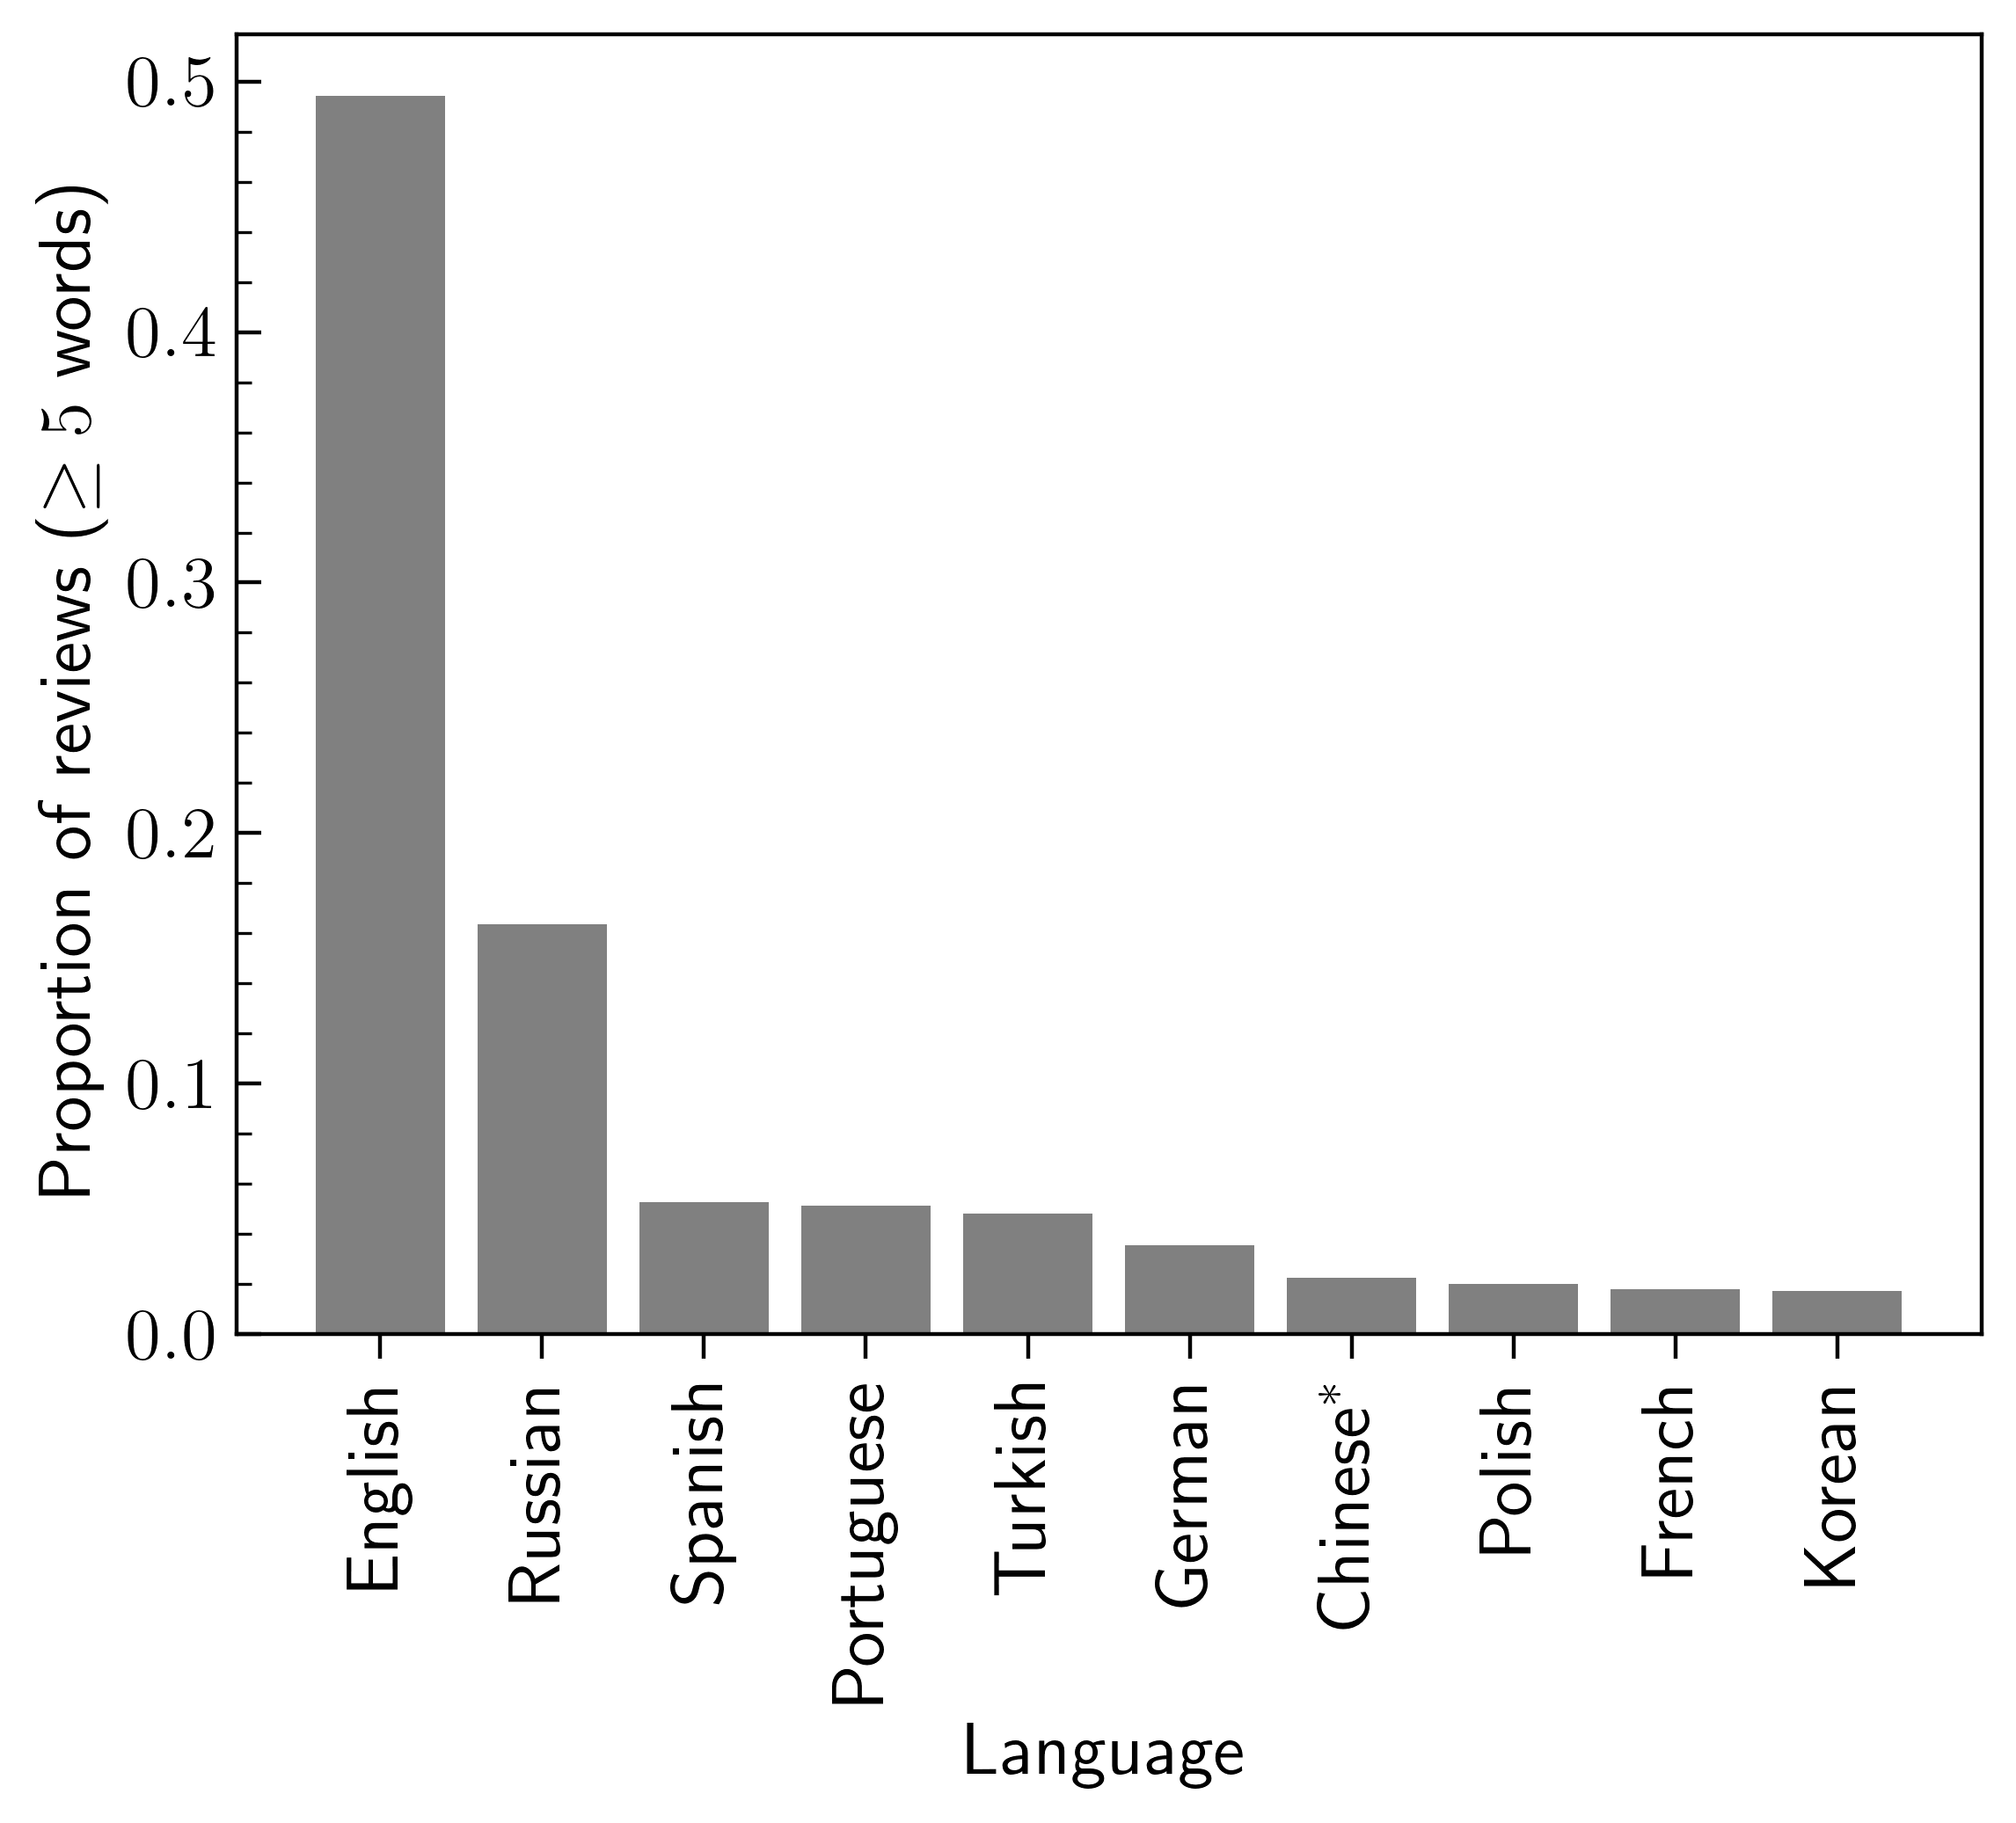
\includegraphics[width=\textwidth]{figures/03_dataset/13_bars_review_langs_min5.png}
        \caption{Reviews with at least five words.}
        \label{fig:Dataset_BarsLangsMin5}
    \end{subfigure}
    \caption{Language reviews were written in.}
    \label{fig:Dataset_BarsLangs}
\end{figure}

\footnotetext[1]{Chinese (Simplified)}

\subsection{Word Count}

The number of words in English-language reviews can be seen in Figure \ref{fig:Dataset_HistWordsEng}. Reviews with more than 277 words, 4.5\% of all such reviews, have been excluded from the histogram. The mean number of words in reviews is 62.7 (\textit{SD} = 134.3) and the median is 20. 25\% of reviews contain 8 words or fewer while 75\% contain 57 words or fewer.

\begin{figure}[ht]
    \centering
    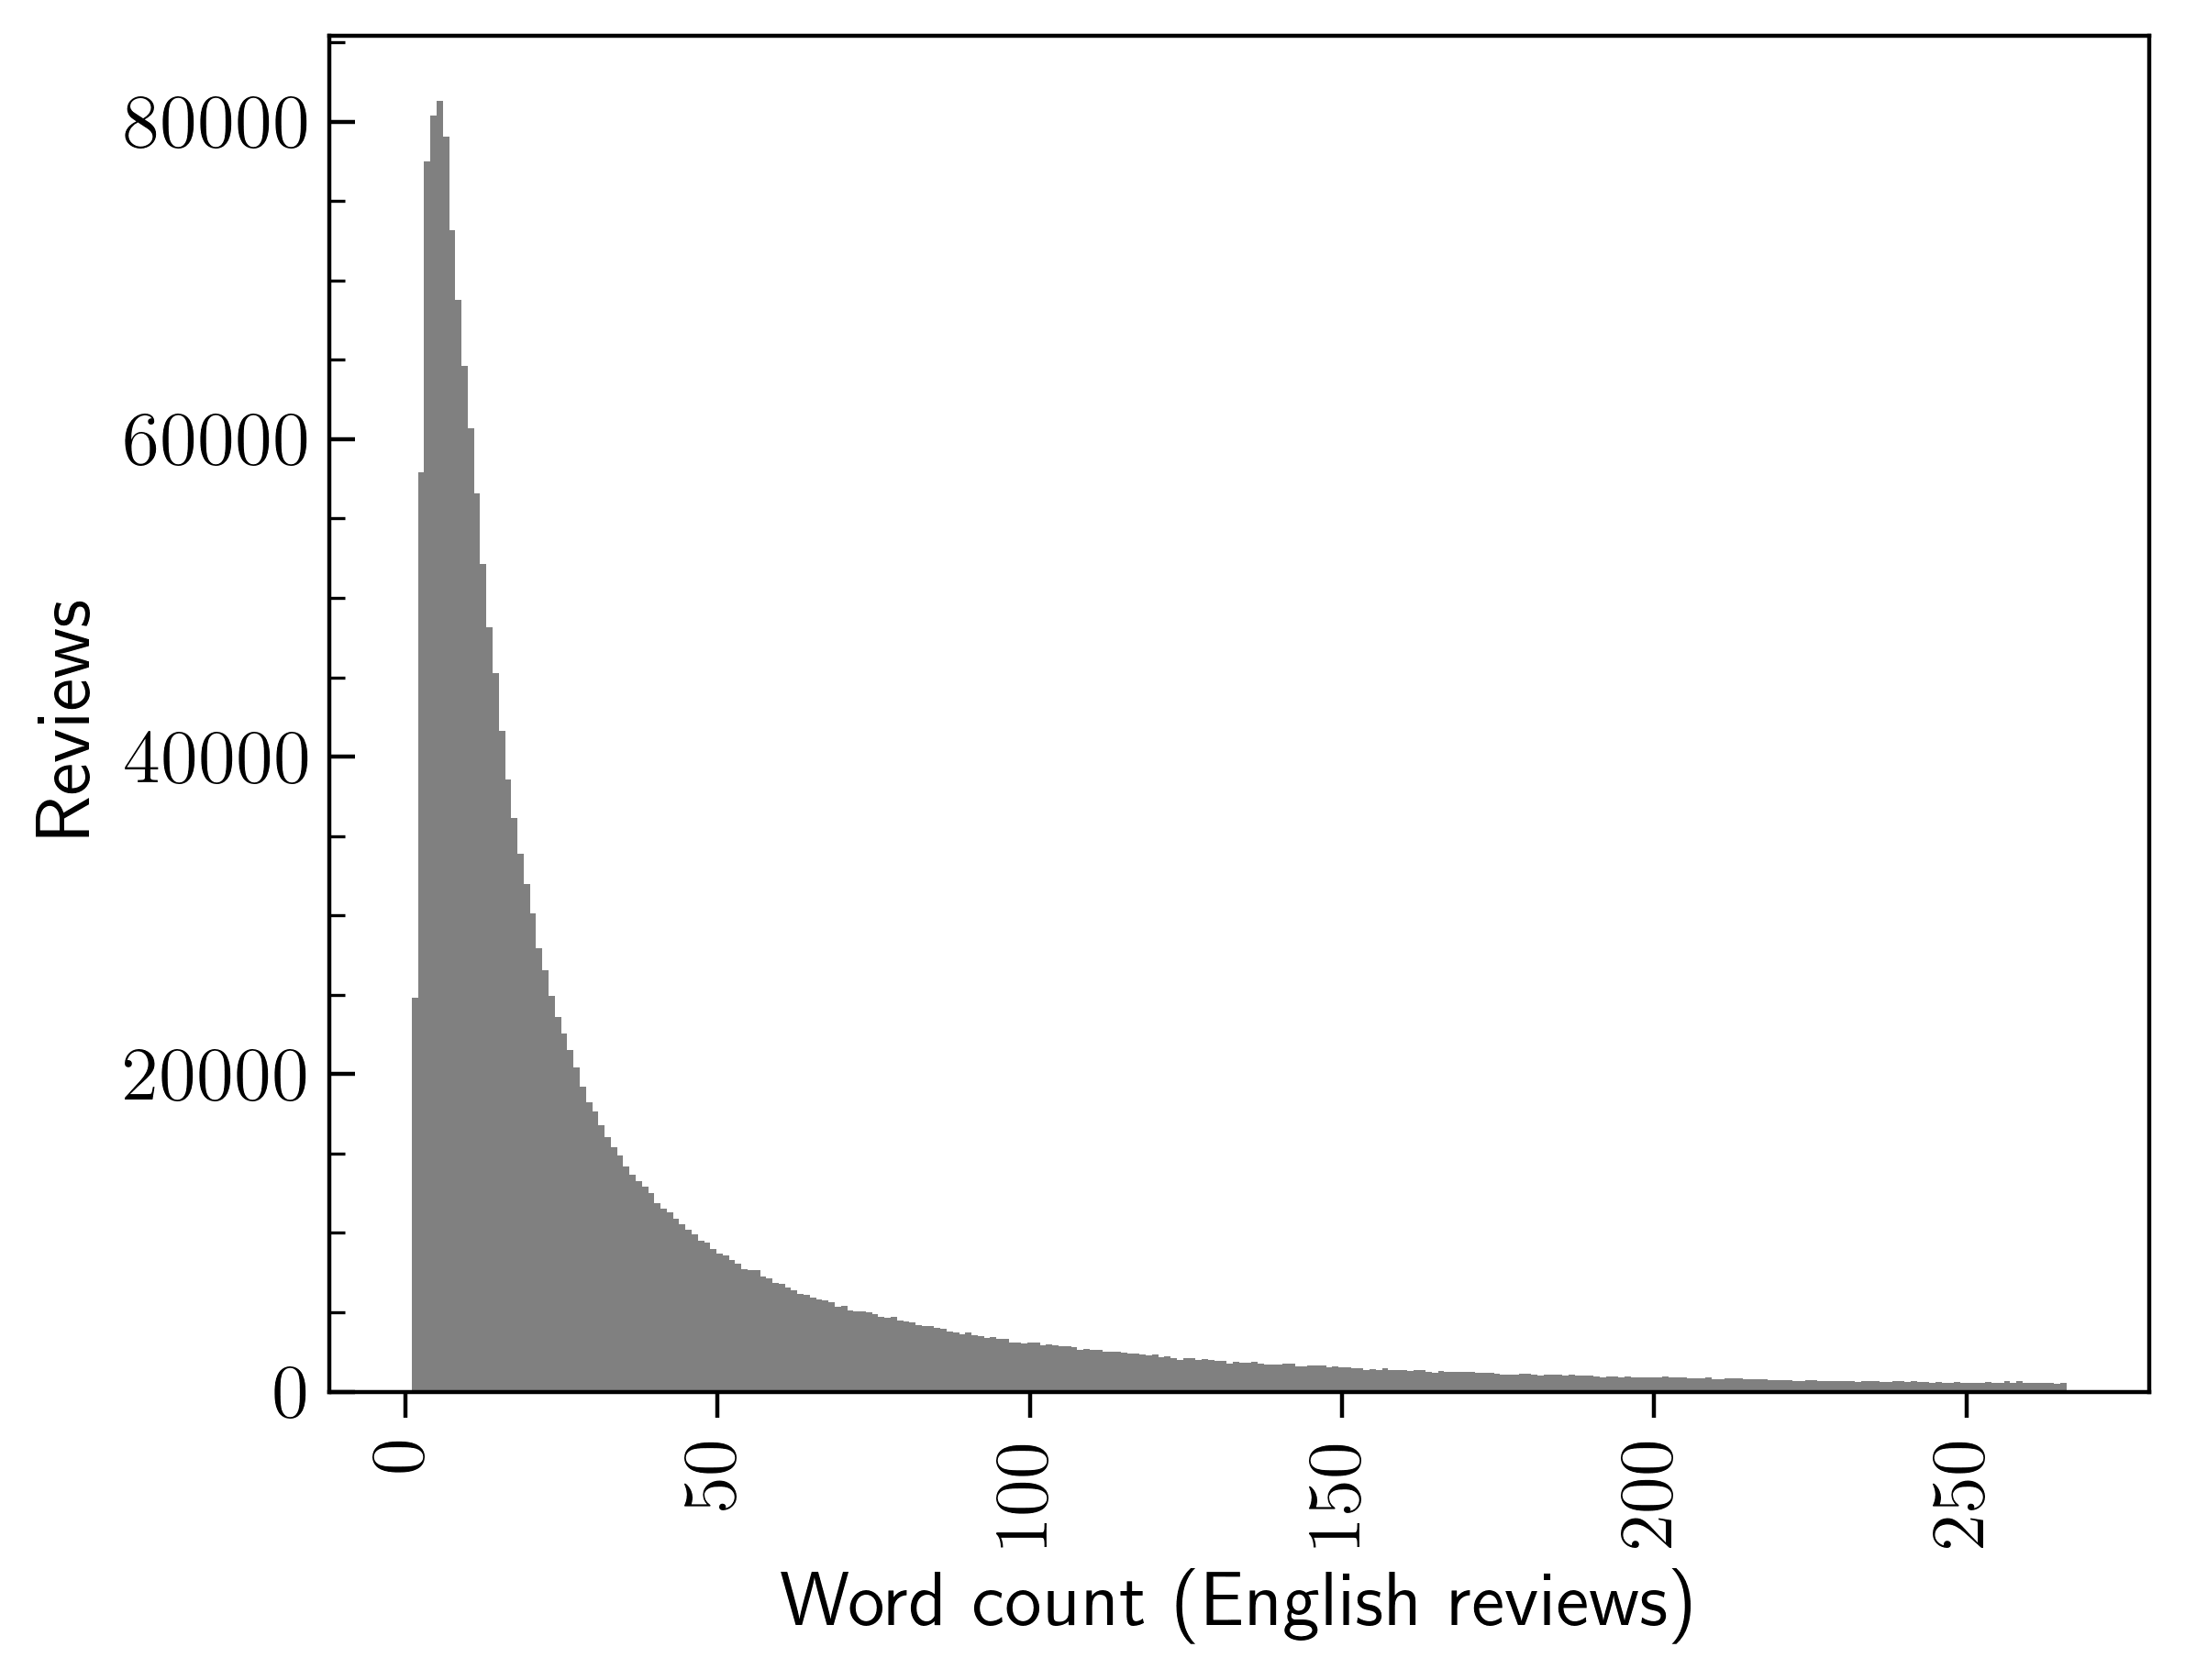
\includegraphics[scale=0.55]{figures/03_dataset/14_hist_review_words_en.png}
    \caption{Word count of English-language reviews.}
    \label{fig:Dataset_HistWordsEng}
\end{figure}
